\section{Tensor Networks Basics}\label{chapter:basics}

As their order increases, representing and working with tensors becomes more complicated. 
Tensor networks provide an efficient framework for working with these high-order objects, simplifying both their representation and analysis. 
The graphical notation of tensor networks offers an intuitive way to visualize and simplify complex tensor operations~\citep{orus2014practical,biamonte2017tensor}. 
In this section, we introduce basic notions on tensors and common tensor operations using the language of tensor networks.

\subsection{What are Tensor Networks?}
As their name suggests, Tensor Networks (TNs) are simply tensors connected to each other to form a network. More precisely, a tensor network is a graph in which vertices represent \emph{tensors} and edges represent \emph{contracted} indices (shared modes). The graphical notation for tensor networks was first introduced by~\cite{penrose1971applications}. Tensors are represented by shapes with legs~(edges), i.e.,
$
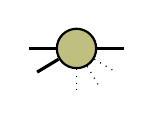
\begin{tikzpicture}[baseline=-0.5ex]
    \tikzset{tensor/.style = {minimum size = 0.5cm,shape = circle,thick,draw=black,inner sep = 0pt}, edge/.style = {thick,line width=.4mm},every loop/.style={}}
    \def\x{6}
    \node[tensor,fill=green!50!red!50!white] (T) at (\x,0) {$\Tt$};
    \draw[edge] (T) -- (\x-0.6,0);
    \draw[edge] (T) -- (\x+0.6,0);
    \draw[edge] (T) -- (\x-0.5,-0.3);
    \draw[dotted] (T) -- (\x,-0.6);
    \draw[dotted] (T) -- (\x+0.5,-0.3);
    \draw[dotted] (T) -- (\x+0.3,-0.5);
    \end{tikzpicture}.
$
We will use different shapes, such as rectangles, triangles, or circles, and various colors to represent tensors. Shapes and colors serve mainly as visual cues. 
The \emph{order} of a tensor is its number of dimensions, e.g., an $N$-th order tensor $\Tt\in\RR^{d_1\times\cdots\times d_N}$ is a multidimensional array of scalars~$\Tt_{i_1,\dots,i_N}$ indexed by $N$ indices $i_1\in [d_1], i_2\in[d_2],\cdots, i_N \in [d_N]$. Each axis is called a \emph{mode} of a tensor: an $N$-th order tensor has $N$ modes.
 
 Tensors naturally generalize vectors and matrices to higher-order arrays. As the order increases, representing these arrays becomes more challenging. \emph{Tensor networks} provide a simple and intuitive way to represent and manipulate these higher-order objects. Complex operations on tensors can be represented more easily with graphical notations of tensor networks~\citep{biamonte2017tensor,orus2014practical}. 


\paragraph{Tensor Network Nodes}\label{def:tn-nodes}
In a tensor network, each node~(or vertex) represents a tensor, and the number of legs~(incident edges) corresponds to the order of the tensor: scalars are nodes with no edges, vector nodes have a single edge, matrix nodes have two edges, and so on. For example,
\begin{center}
    
    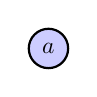
\begin{tikzpicture}[baseline=-0.5ex]
    \tikzset{tensor/.style = {minimum size = 0.5cm,shape = circle,thick,draw=black,inner sep = 0pt}, edge/.style = {thick,line width=.4mm},every loop/.style={}}
    \def\y{0}
    \def\x{0}
    \node[tensor,fill=blue!20!white] (a) at (\x,\y){\scalebox{0.85}{$a$}};
    \end{tikzpicture}%
    \ \ \ $\in \RR$,\hspace{0.01cm}
    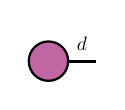
\begin{tikzpicture}[baseline=-0.5ex]
    \tikzset{tensor/.style = {minimum size = 0.5cm,shape = circle,thick,draw=black,inner sep = 0pt}, edge/.style = {thick,line width=.4mm},every loop/.style={}}
    \def\y{0}
    \def\x{0}
    \node[tensor,fill=blue!40!red!60!white] (a) at (\x,\y){\scalebox{0.85}{$\ab$}};
    \draw[edge] (\x+0.25,\y) -- (\x+0.6,\y)  node [midway,above] {\scalebox{0.7}{\dimcolor{$d$}}};
    \end{tikzpicture}
    $\in \RR^d$,\hspace{0.3cm}
    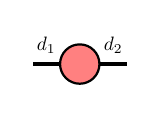
\begin{tikzpicture}[baseline=-0.5ex]
    \tikzset{tensor/.style = {minimum size = 0.5cm,shape = circle,thick,draw=black,inner sep = 0pt}, edge/.style = {thick,line width=.4mm},every loop/.style={}}
    \def\y{0}
    \def\x{0}
    \node[tensor,fill=red!50!white] (A) at (\x,\y){\scalebox{0.85}{$\Ab$}};
    \draw[edge] (\x+0.25,\y) -- (\x+0.6,\y)  node [midway,above] {\scalebox{0.7}{\dimcolor{$d_2$}}};
    \draw[edge] (\x-0.25,\y) -- (\x-0.6,\y)  node [midway,above] {\scalebox{0.7}{\dimcolor{$d_1$}}};
    \end{tikzpicture}
    \ \ \ $\in \RR^{d_1\times d_2}$,\hspace{0.3cm}
    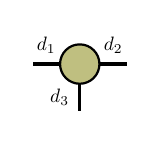
\begin{tikzpicture}[baseline=-0.5ex]
    \tikzset{tensor/.style = {minimum size = 0.5cm,shape = circle,thick,draw=black,inner sep = 0pt}, edge/.style = {thick,line width=.4mm},every loop/.style={}}
    \def\y{0}
    \def\x{0}
    \node[tensor,fill=green!50!red!50!white] (A) at (\x,\y){\scalebox{0.85}{$\At$}};
    \draw[edge] (\x+0.25,\y) -- (\x+0.6,\y)  node [midway,above] {\scalebox{0.7}{\dimcolor{$d_2$}}};
    \draw[edge] (\x-0.25,\y) -- (\x-0.6,\y)  node [midway,above] {\scalebox{0.7}{\dimcolor{$d_1$}}};
    \draw[edge] (\x,\y-0.25) -- (\x,\y-0.6)  node [midway,left] {\scalebox{0.7}{\dimcolor{$d_3$}}};
    \end{tikzpicture}
    \ \ \ $\in \RR^{d_1\times d_2\times d_3}$,\hspace{0.01cm}
    \begin{tikzpicture}[baseline=-0.5ex]
    \tikzset{tensor/.style = {minimum width = 1.8cm,minimum height = 0.4cm,shape = rounded rectangle,thick,draw=black,inner sep = 0pt}, edge/.style = {thick,line width=.4mm},every loop/.style={}}
    \def\x{0}
    \def\y{0}
    \draw[edge] (\x-0.2,\y-0.15) -- (\x-0.2,\y-0.6)node [midway,left=-0.05cm] {\scalebox{0.7}{\dimcolor{$d_2$}}};
    \draw[edge] (\x-0.6,\y-0.15) -- (\x-0.6,\y-0.6)node [midway,left=-0.05cm] {\scalebox{0.7}{\dimcolor{$d_1$}}};
    \draw[edge] (\x+0.2,\y-0.15) -- (\x+0.2,\y-0.6)node [midway,left=-0.05cm] {\scalebox{0.7}{\dimcolor{$d_3$}}};
    \draw[edge] (\x+0.6,\y-0.15) -- (\x+0.6,\y-0.6)node [midway,left=-0.05cm] {\scalebox{0.7}{\dimcolor{$d_4$}}};
    \node[tensor,fill=green!30!white] (Bt) at (\x,\y){$\Bt$};
    \end{tikzpicture}
    $\in \RR^{d_1\times d_2\times d_3\times d_4}$.

\end{center}
represent a scalar, a vector, a matrix, a third- and a fourth-order tensors, respectively. 
Throughout this manuscript,
\begin{itemize}
    \item Tensors are represented by colored shapes called nodes, where the colors and shapes have no specific meaning~(unless stated otherwise). 
    \item We use lower case letters for scalars~(e.g., $a$), bold lower case letters for vectors~(e.g., $\vb$), bold upper case letters for matrices (e.g., $\Mb$), and 
    bold upper case calligraphic letters for higher-order tensors~(e.g., $\Tt$).
    \item The dimension of each mode of a tensor is depicted by a gray letter positioned at the top of the corresponding leg, e.g., 
$
    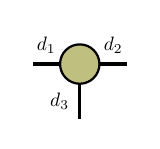
\begin{tikzpicture}[baseline=-0.5ex]
    \tikzset{tensor/.style = {minimum size = 0.5cm,shape = circle,thick,draw=black,inner sep = 0pt}, edge/.style = {thick,line width=.4mm},every loop/.style={}}
    \def\y{0}
    \def\x{0}
    \node[tensor,fill=green!50!red!50!white] (A) at (\x,\y){\scalebox{0.85}{$\At$}};
    \draw[edge] (\x+0.25,\y) -- (\x+0.6,\y)  node [midway,above] {\scalebox{0.7}{\dimcolor{$d_2$}}};
    \draw[edge] (\x-0.25,\y) -- (\x-0.6,\y)  node [midway,above] {\scalebox{0.7}{\dimcolor{$d_1$}}};
    \draw[edge] (\x,\y-0.25) -- (\x,\y-0.7)  node [midway,left] {\scalebox{0.7}{\dimcolor{$d_3$}}};
    \end{tikzpicture}
    \ \ \ \in \RR^{d_1\times d_2\times d_3},
$
is a third-order tensor of size $d_1\times d_2\times d_3$.
    
$
\At_{i,j,k} = 
    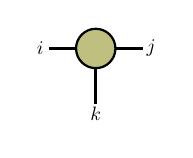
\begin{tikzpicture}[baseline=-0.5ex]
    \tikzset{tensor/.style = {minimum size = 0.5cm,shape = circle,thick,draw=black,inner sep = 0pt}, edge/.style = {thick,line width=.4mm},every loop/.style={}}
    \def\y{0}
    \def\x{0}
    \node[tensor,fill=green!50!red!50!white] (A) at (\x,\y){\scalebox{0.85}{$\At$}};
    \draw[edge] (\x+0.25,\y) -- (\x+0.6,\y)  node [pos=1.3] {\scalebox{0.7}{\indcolor{$j$}}};
    \draw[edge] (\x-0.25,\y) -- (\x-0.6,\y)  node [pos=1.3] {\scalebox{0.7}{\indcolor{$i$}}};
    \draw[edge] (\x,\y-0.25) -- (\x,\y-0.7)  node [pos=1.3] {\scalebox{0.7}{\indcolor{$k$}}};
    \end{tikzpicture}
$    
is the $(i,j,k)$-th element of the third-order tensor $\At$.
\end{itemize}
Note that large matrices can sometimes be viewed as high-order tensors through reshaping, e.g., 
\begin{align*}
    &\Tb
    =
    \begin{tikzpicture}[baseline=\baseline]
    \tikzset{tensor/.style = {minimum size = 0.5cm,shape = circle,thick,draw=black,inner sep = 0pt}, edge/.style = {thick,line width=.4mm},every loop/.style={}}
    \def\x{0}
    \def\y{0}
    \node[tensor,fill=green!50!blue!40!white] (Tb) at (\x,\y){$\Tb$};
    \draw[edge] (Tb) -- (\x+1.15,\y) node [midway,above] {\scalebox{0.7}{\dimcolor{$J_1J_2J_3J_4$}}};
    \draw[edge] (Tb) -- (\x-1.15,\y) node [midway,above] {\scalebox{0.7}{\dimcolor{$I_1I_2I_3I_4$}}};
    \end{tikzpicture}\in\RR^{I_1I_2I_3I_4\times J_1J_2J_3J_4}
    \equiv
    \Tt = 
    \begin{tikzpicture}[baseline=-0.5ex]
    \tikzset{tensor/.style = {minimum width = 1.8cm,minimum height = 0.4cm,shape = rounded rectangle,thick,draw=black,inner sep = 0pt}, edge/.style = {thick,line width=.4mm},every loop/.style={}}
    \def\x{0}
    \def\y{0}
    \draw[edge] (\x-0.2,\y-0.15) -- (\x-0.2,\y-0.6)node [midway,left=-0.05cm] {\scalebox{0.7}{\dimcolor{$I_2$}}};
    \draw[edge] (\x-0.6,\y-0.15) -- (\x-0.6,\y-0.6)node [midway,left=-0.05cm] {\scalebox{0.7}{\dimcolor{$I_1$}}};
    \draw[edge] (\x+0.2,\y-0.15) -- (\x+0.2,\y-0.6)node [midway,left=-0.05cm] {\scalebox{0.7}{\dimcolor{$I_3$}}};
    \draw[edge] (\x+0.6,\y-0.15) -- (\x+0.6,\y-0.6)node [midway,left=-0.05cm] {\scalebox{0.7}{\dimcolor{$I_4$}}};
    \draw[edge] (\x-0.2,\y+0.15) -- (\x-0.2,\y+0.6)node [midway,left=-0.05cm] {\scalebox{0.7}{\dimcolor{$J_2$}}};
    \draw[edge] (\x-0.6,\y+0.15) -- (\x-0.6,\y+0.6)node [midway,left=-0.05cm] {\scalebox{0.7}{\dimcolor{$J_1$}}};
    \draw[edge] (\x+0.2,\y+0.15) -- (\x+0.2,\y+0.6)node [midway,left=-0.05cm] {\scalebox{0.7}{\dimcolor{$J_3$}}};
    \draw[edge] (\x+0.6,\y+0.15) -- (\x+0.6,\y+0.6)node [midway,left=-0.05cm] {\scalebox{0.7}{\dimcolor{$J_4$}}};
    \node[tensor,fill=yellow] (Bt) at (\x,\y){$\Tt$};
    \end{tikzpicture}
    \in\RR^{I_1\times I_2\times I_3\times I_4\times J_1 \times J_2\times J_3\times J_4}.
\end{align*}
\paragraph{Tensor Network Edges}\label{subsec:contraction} In tensor network diagram, legs are of two types: contracted legs~(those connecting two tensors) and un-contracted legs, also called free legs, with one dangling end~(i.e., a leg that is not connected to any other tensor). As mentioned above, un-contracted legs correspond to free indices:  the number of free legs indicates the order of a tensor: scalars have no free legs, vectors have one, matrices have two, and higher-order tensors have three or more.  Contracted legs represent contractions: 
tensors can be connected along legs of the same size, which represents a summation~(contraction) over the connected modes. 
We use the terms summation and contraction interchangeably. The most common contraction operation is \textit{matrix multiplication}. For two matrices $\Ab\in\RR^{d_1\times R}, \Bb\in\RR^{R\times d_2}$, their matrix product corresponds to a contraction between the second mode of $\Ab$ and the first mode of $\Bb$:

\begin{align}\label{eq:matrix-product}
(\Ab\Bb)_{ij} 
=
\begin{tikzpicture}[baseline=\baseline]
   \tikzset{tensor/.style = {minimum size = 0.5cm,shape = circle,thick,draw=black,inner sep = 0pt}, edge/.style = {thick,line width=.4mm},every loop/.style={}}
    \def\y{0}
    \def\x{0}
    \node[tensor,fill=red!50!white] (A) at (\x,\y){\scalebox{0.85}{$\Ab$}};
    \node[tensor,fill=blue!50!white] (B) at (\x+1,\y){\scalebox{0.85}{$\Bb$}};
    \draw[edge] (A) -- (B) node [above,midway] {\scalebox{0.7}{\dimcolor{$R$}}};
    \draw[edge] (\x-0.25,\y) -- (\x-0.75,\y)  node [pos=1.3] {\scalebox{0.7} {\indcolor{$i$}}};
    \draw[edge] (\x+1.25,\y) -- (\x+1.75,\y)  node [pos=1.3] {\scalebox{0.7}{\indcolor{$j$}}};
    \end{tikzpicture}
= \sum_{r=1}^R\Ab_{ir}\Bb_{rj},\ \ \ \text{for}\ \ i\in[d_1],j\in[d_2]\ .
\end{align}
Since this equality is true for all indices $i$ and $j$, we can simply write
\begin{align}\label{eq:matrix-product_noidx}
\Ab\Bb 
=
\begin{tikzpicture}[baseline=\baseline]
   \tikzset{tensor/.style = {minimum size = 0.5cm,shape = circle,thick,draw=black,inner sep = 0pt}, edge/.style = {thick,line width=.4mm},every loop/.style={}}
    \def\y{0}
    \def\x{0}
    \node[tensor,fill=red!50!white] (A) at (\x,\y){\scalebox{0.85}{$\Ab$}};
    \node[tensor,fill=blue!50!white] (B) at (\x+1,\y){\scalebox{0.85}{$\Bb$}};
    \draw[edge] (A) -- (B) node [above,midway] {\scalebox{0.7}{\dimcolor{$R$}}};
    \draw[edge] (\x-0.25,\y) -- (\x-0.75,\y)  node [midway, above] {\scalebox{0.7}{\dimcolor{$d_1$}}};
    \draw[edge] (\x+1.25,\y) -- (\x+1.75,\y)  node [midway,above] {\scalebox{0.7}{\dimcolor{$d_2$}}};
    \end{tikzpicture}
 \ \in \mathbb R^{d_1\times d_2}.
\end{align}

 In the above diagram, we can see that there is a connection between the legs of the same size $R$. This is consistent with matrix multiplication where there is a sum over indices with the same dimension. Finally, since the resulting diagram has two free legs, it represents a matrix. Here, the final object is a matrix which can be represented as  a single node, demonstrating how nodes can be merged in tensor networks:
$$
\Ab\Bb =\Mb \Leftrightarrow 
\begin{tikzpicture}[baseline=\baseline]
   \tikzset{tensor/.style = {minimum size = 0.5cm,shape = circle,thick,draw=black,inner sep = 0pt}, edge/.style = {thick,line width=.4mm},every loop/.style={}}
    \def\y{0}
    \def\x{0}
    \node[tensor,fill=red!50!white] (A) at (\x,\y){\scalebox{0.85}{$\Ab$}};
    \node[tensor,fill=blue!50!white] (B) at (\x+1,\y){\scalebox{0.85}{$\Bb$}};
    \draw[edge] (A) -- (B) node [above,midway] {\scalebox{0.7}{\dimcolor{$R$}}};
    \draw[edge] (\x-0.25,\y) -- (\x-0.75,\y)  node [midway, above] {\scalebox{0.7}{\dimcolor{$d_1$}}};
    \draw[edge] (\x+1.25,\y) -- (\x+1.75,\y)  node [midway,above] {\scalebox{0.7}{\dimcolor{$d_2$}}};
    \node[draw=none] () at (\x+2,\y) {\scalebox{1}{\textcolor{black}{$=$}}};
    \node[tensor,fill=blue!30!red!20!white] (M) at (\x+3,\y){\scalebox{0.85}{$\Mb$}};
    \draw[edge] (M) -- (\x+3.75,\y)  node [midway,above] {\scalebox{0.7}{\dimcolor{$d_2$}}};
    \draw[edge] (M) -- (\x+2.25,\y)  node [midway,above] {\scalebox{0.7}{\dimcolor{$d_1$}}};
    \end{tikzpicture}.
$$
Contraction between two matrices can directly be extended to contractions between a matrix and a vector, a tensor and a matrix, a tensor a matrix and a vector products, etc. Here are some examples of tensor networks with their corresponding mathematical expressions: 
\begin{align}\label{eq:matvec}
\Ab\in\RR^{d_1\times R},\vb\in\RR^{R} \ : \ \
\begin{tikzpicture}[baseline=\baseline]
   \tikzset{tensor/.style = {minimum size = 0.5cm,shape = circle,thick,draw=black,inner sep = 0pt}, edge/.style = {thick,line width=.4mm},every loop/.style={}}
    \def\y{0}
    \def\x{0}
    \node[tensor,fill=red!50!white] (A) at (\x,\y){\scalebox{0.85}{$\Ab$}};
    \node[tensor,fill=blue!10!white] (v) at (\x+1,\y){\scalebox{0.85}{$\vb$}};
    \draw[edge] (A) -- (v) node [above,midway] {\scalebox{0.7}{\dimcolor{$R$}}};
    \draw[edge] (\x-0.25,\y) -- (\x-0.75,\y)  node [pos=1.3]{\scalebox{0.7}{\indcolor{$i$}}};
    \end{tikzpicture}
=\sum_{r=1}^R\Ab_{ir}\vb_r,
\end{align}
\begin{align}\label{eq:tenmat}
\At\in\RR^{d_1\times R\times d_2},\Ab\in\RR^{R\times d_3}\ :\ \
\begin{tikzpicture}[baseline = \baseline]
    \tikzset{tensor/.style = {minimum size = 0.5cm,shape = circle,thick,draw=black,inner sep = 0pt}, edge/.style = {thick,line width=.4mm},every loop/.style={}}
    \def\y{0}
    \def\x{0}
    \node[tensor,fill=green!50!red!50!white] (At) at (\x,\y){\scalebox{0.85}{$\At$}};
    \node[tensor,fill=red!50!white] (A) at (\x+1,\y){\scalebox{0.85}{$\Ab$}};
    \draw[edge] (At) -- (A) node [above,midway] {\scalebox{0.7}{\dimcolor{$R$}}};
    \draw[edge] (\x-0.25,\y) -- (\x-0.75,\y)  node [pos=1.3] {\scalebox{0.7}{\indcolor{$i$}}};
    \draw[edge] (\x,\y-0.25) -- (\x,\y-0.75)  node [pos=1.3] {\scalebox{0.7}{\indcolor{$j$}}};
    \draw[edge] (\x+1.25,\y) -- (\x+1.75,\y)  node [pos=1.3] {\scalebox{0.7}{\indcolor{$k$}}};
\end{tikzpicture} 
= \sum_{r=1}^R\At_{ijr}\Ab_{rk},
\end{align}
\begin{align}\label{eq:tenmatvec}
\At\in\RR^{d_1\times R\times d_2},\Ab\in\RR^{R\times d_3}, \vb\in\RR^{d_3}&:
   \begin{tikzpicture}[baseline = \baseline]
    \tikzset{tensor/.style = {minimum size = 0.5cm,shape = circle,thick,draw=black,inner sep = 0pt}, edge/.style = {thick,line width=.4mm},every loop/.style={}}
    \def\y{0}
    \def\x{0}
    \node[tensor,fill=green!50!red!50!white] (At) at (\x,\y){\scalebox{0.85}{$\At$}};
    \node[tensor,fill=red!50!white] (A) at (\x+1,\y){\scalebox{0.85}{$\Ab$}};
    \node[tensor,fill=blue!40!red!60!white] (a) at (\x+2,\y){\scalebox{0.85}{$\vb$}};
    \draw[edge] (At) -- (A) node [above,midway] {\scalebox{0.7}{\dimcolor{$R$}}};
    \draw[edge] (A) -- (a) node [above,midway] {\scalebox{0.7}{\dimcolor{$d_3$}}};
    \draw[edge] (\x-0.25,\y) -- (\x-0.75,\y)  node [pos=1.3] {\scalebox{0.7}{\indcolor{$i$}}};
    \draw[edge] (\x,\y-0.25) -- (\x,\y-0.75)  node [pos=1.3] {\scalebox{0.7}{\indcolor{$j$}}};
    \end{tikzpicture} 
= \sum_{r=1}^R\sum_{k=1}^{d_3}\At_{ijr}\Ab_{rk}\ab_{k}.
\end{align}
As we can see in all diagrams above, edges between two nodes represent summations. They also indicate that two tensors share dimensions of the same size on the corresponding mode. 
As explained before, the number of free legs in the tensor network corresponds to the order of the tensor it represents. For the previous examples, we have

$$
\begin{tikzpicture}[baseline=\baseline]
   \tikzset{tensor/.style = {minimum size = 0.5cm,shape = circle,thick,draw=black,inner sep = 0pt}, edge/.style = {thick,line width=.4mm},every loop/.style={}}
    \def\y{0}
    \def\x{0}
    \node[tensor,fill=red!50!white] (A) at (\x,\y){\scalebox{0.85}{$\Ab$}};
    \node[tensor,fill=blue!10!white] (v) at (\x+1,\y){\scalebox{0.85}{$\vb$}};
    \draw[edge] (A) -- (v) node [above,midway] {\scalebox{0.7}{\dimcolor{$R$}}};
    \draw[edge] (\x-0.25,\y) -- (\x-0.75,\y)  node [midway, above] {\scalebox{0.7}{\dimcolor{$d_1$}}};
    \end{tikzpicture} 
   \in \mathbb R^{d_1},\ \ 
\begin{tikzpicture}[baseline = \baseline]
    \tikzset{tensor/.style = {minimum size = 0.5cm,shape = circle,thick,draw=black,inner sep = 0pt}, edge/.style = {thick,line width=.4mm},every loop/.style={}}
    \def\y{0}
    \def\x{0}
    \node[tensor,fill=green!50!red!50!white] (At) at (\x,\y){\scalebox{0.85}{$\At$}};
    \node[tensor,fill=red!50!white] (A) at (\x+1,\y){\scalebox{0.85}{$\Ab$}};
    \draw[edge] (At) -- (A) node [above,midway] {\scalebox{0.7}{\dimcolor{$R$}}};
    \draw[edge] (\x-0.25,\y) -- (\x-0.75,\y)  node [midway,above] {\scalebox{0.7}{\dimcolor{$d_1$}}};
    \draw[edge] (\x,\y-0.25) -- (\x,\y-0.75)  node [midway,left] {\scalebox{0.7}{\dimcolor{$d_2$}}};
    \draw[edge] (\x+1.25,\y) -- (\x+1.75,\y)  node [midway,above] {\scalebox{0.7}{\dimcolor{$d_3$}}};
\end{tikzpicture} 
\in \mathbb R^{d_1\times d_2 \times d_3},\ \ \text{and}\ \ 
    \begin{tikzpicture}[baseline = \baseline]
    \tikzset{tensor/.style = {minimum size = 0.5cm,shape = circle,thick,draw=black,inner sep = 0pt}, edge/.style = {thick,line width=.4mm},every loop/.style={}}
    \def\y{0}
    \def\x{0}
    \node[tensor,fill=green!50!red!50!white] (At) at (\x,\y){\scalebox{0.85}{$\At$}};
    \node[tensor,fill=red!50!white] (A) at (\x+1,\y){\scalebox{0.85}{$\Ab$}};
    \node[tensor,fill=blue!40!red!60!white] (a) at (\x+2,\y){\scalebox{0.85}{$\vb$}};
    \draw[edge] (At) -- (A) node [above,midway] {\scalebox{0.7}{\dimcolor{$R$}}};
    \draw[edge] (A) -- (a) node [above,midway] {\scalebox{0.7}{\dimcolor{$d_3$}}};
    \draw[edge] (\x-0.25,\y) -- (\x-0.75,\y)  node [midway,above] {\scalebox{0.7}{\dimcolor{$d_1$}}};
    \draw[edge] (\x,\y-0.25) -- (\x,\y-0.75)  node [midway,left] {\scalebox{0.7}{\dimcolor{$d_2$}}};
    \end{tikzpicture} 
\in \mathbb R^{d_1\times d_2}.
$$
 
\paragraph{From mathematical expressions to tensor networks, and back} Tensor networks are simple to work with because there are no strict rules for representing legs and nodes. 
In tensor network diagrams, nodes and edges can be positioned arbitrarily in the plane, only the graph structure matters. 
For example, when translating matrix multiplication into  a tensor network diagram, the key feature is to ensure the dimension of the connected legs are consistent, e.g., for $\Ab\in\RR^{d_1\times R}, \Bb\in\RR^{R\times d_2}$  all diagrams below illustrate the \emph{same} matrix multiplication:
\begin{align*} 
\Ab\Bb
=
\begin{tikzpicture}[baseline=\baseline]
   \tikzset{tensor/.style = {minimum size = 0.5cm,shape = circle,thick,draw=black,inner sep = 0pt}, edge/.style = {thick,line width=.4mm},every loop/.style={}}
    \def\y{0}
    \def\x{0}
    \node[tensor,fill=red!50!white] (A) at (\x,\y){\scalebox{0.85}{$\Ab$}};
    \node[tensor,fill=blue!50!white] (B) at (\x+1,\y){\scalebox{0.85}{$\Bb$}};
    \draw[edge] (A) -- (B) node [midway,above] {\scalebox{0.7}{\dimcolor{$R$}}};;
    \draw[edge] (\x-0.25,\y) -- (\x-0.75,\y) node [midway,above] {\scalebox{0.7}{\dimcolor{$d_1$}}};;
    \draw[edge] (\x+1.25,\y) -- (\x+1.75,\y) node [midway,above] {\scalebox{0.7}{\dimcolor{$d_2$}}};;
    \node[draw=none] () at (\x+1.95,\y) {$=$};
    \node[tensor,fill=red!50!white] (A1) at (\x+2.85,\y){\scalebox{0.85}{$\Ab$}};
    \node[tensor,fill=blue!50!white] (B1) at (\x+3.85,\y){\scalebox{0.85}{$\Bb$}};
    \draw[edge] (A1) -- (B1) node [midway,above] {\scalebox{0.7}{\dimcolor{$R$}}};;
    \draw[edge] (A1) to [out=60,in=60, distance=0.5cm] (\x+2.2,\y);
    \draw[edge] (B1) to [out=60,in=60, distance=0.5cm] (\x+4.4,\y-0.5);
    \node[draw=none] () at (\x+2.4,\y+0.65) {\scalebox{0.7}{\dimcolor{$d_1$}}};
    \node[draw=none] () at (\x+4,\y+0.65) {\scalebox{0.7}{\dimcolor{$d_2$}}};
    \node[draw=none] () at (\x+4.7,\y) {$=$};
    \node[tensor,fill=blue!50!white] (A2) at (\x+5.3,\y){\scalebox{0.85}{$\Bb$}};
    \node[tensor,fill=red!50!white] (B2) at (\x+6.3,\y){\scalebox{0.85}{$\Ab$}};
    \draw[edge] (A2) -- (B2) node [midway,above] {\scalebox{0.7}{\dimcolor{$R$}}};;
    \draw[edge] (A2) -- (\x+5.3,\y+0.75) node [midway,left] {\scalebox{0.7}{\dimcolor{$d_2$}}};
     \draw[edge] (B2) -- (\x+6.3,\y-0.75) node [midway,right] {\scalebox{0.7}{\dimcolor{$d_1$}}};   
     \node[draw=none] () at (\x+7.1,\y) {$=$};
    \node[tensor,fill=red!50!white] (A3) at (\x+7.6,\y+0.5){\scalebox{0.85}{$\Ab$}};
    \node[tensor,fill=blue!50!white] (B3) at (\x+7.6,\y-0.5){\scalebox{0.85}{$\Bb$}};
    \draw[edge] (A3) -- (B3) node [midway,right] {\scalebox{0.7}{\dimcolor{$R$}}};
    \draw[edge] (A3) -- (\x+7.6,\y+1.25) node [midway,left] {\scalebox{0.7}{\dimcolor{$d_1$}}};
    \draw[edge] (B3) -- (\x+7.6,\y-1.25) node [midway,left] {\scalebox{0.7}{\dimcolor{$d_2$}}};
    \end{tikzpicture}.
\end{align*}
Note that because of the sizes of $\Ab\in\RR^{d_1\times R}$ and $\Bb\in\RR^{R\times d_2}$, there is only one way to do the contraction between the two; hence, there would be no ambiguity in the diagrams above even if we omitted the dimensions on the edges. 

Conversely, translating tensor network diagrams into mathematical formulations can lead to multiple interpretations. For example, the following matrix multiplication diagram
$
\begin{tikzpicture}[baseline=\baseline]
   \tikzset{tensor/.style = {minimum size = 0.5cm,shape = circle,thick,draw=black,inner sep = 0pt}, edge/.style = {thick,line width=.4mm},every loop/.style={}}
    \def\y{0}
    \def\x{0}
    \node[tensor,fill=red!50!white] (A) at (\x,\y){\scalebox{0.85}{$\Ab$}};
    \node[tensor,fill=blue!50!white] (B) at (\x+1,\y){\scalebox{0.85}{$\Bb$}};
    \draw[edge] (A) -- (B) node [midway,above] {\scalebox{0.7}{\dimcolor{$R$}}};
    \draw[edge] (\x-0.25,\y) -- (\x-0.75,\y) node [midway,above] {\scalebox{0.7}{\dimcolor{$d_1$}}};
    \draw[edge] (\x+1.25,\y) -- (\x+1.75,\y) node [midway,above] {\scalebox{0.7}{\dimcolor{$d_2$}}};
\end{tikzpicture}
$
can be interpreted differently depending on what we choose the shapes of $\Ab$, $\Bb$ and the resulting matrix to be:
\begin{itemize}
    \item if $\Ab\in\RR^{d_1\times R}, \Bb\in\RR^{R\times d_2}$ and the result is of size $d_1 \times d_2$, then the diagram represents the product $\Ab\Bb$,
    \item if $\Ab\in\RR^{R\times d_1}, \Bb\in\RR^{R\times d_2}$ and the result is of size $d_1 \times d_2$, then the diagram represents the product $\Ab^\ts\Bb$,
    \item if $\Ab\in\RR^{R\times d_1}, \Bb\in\RR^{R\times d_2}$ and the result is of size $d_2 \times d_1$, then the diagram represents the product $\Bb^\ts\Ab$,
    \item ...
\end{itemize}
Therefore, one should be mindful when translating tensor network diagrams into mathematical formulations. But this is also what makes tensor networks very useful! When we are working with the diagrams, rather than mathematical expressions, we do not need to care about, e.g., transposes.

\paragraph{Contracting two legs of the same node. } As explained previously, any two legs of the same dimension can be connected to form an edge in a tensor network, even two legs corresponding to the same node. Consider for example a fifth-order tensor $\Tt\in\mathbb R^{d_1\times d_2 \times d_3 \times d_2 \times d_4}$. Since its 2nd and 4th modes have the same dimension, we can contract them together. Since the resulting tensor network has 3 dangling legs, it represents a third-order tensor: 
\begin{align*}
&\begin{tikzpicture}[baseline=-0.5ex]
    \tikzset{tensor/.style = {minimum width = 1.8cm,minimum height = 0.4cm,shape = rounded rectangle,thick,draw=black,inner sep = 0pt}, edge/.style = {thick,line width=.4mm},every loop/.style={}}
    \def\x{0}
    \def\y{0}
    \draw[edge] (\x-0.4,\y-0.15) -- (\x-0.4,\y-0.5)node [near end,left=-0.05cm] {\scalebox{0.7}{\dimcolor{$d_2$}}};
    \draw[edge] (\x-0.8,\y-0.15) -- (\x-0.8,\y-0.5)node [near end,left=-0.05cm] {\scalebox{0.7}{\dimcolor{$d_1$}}};
    \draw[edge] (\x,\y-0.15) -- (\x,\y-0.5)node [near end,left=-0.05cm] {\scalebox{0.7}{\dimcolor{$d_3$}}};
    \draw[edge] (\x+0.4,\y-0.15) -- (\x+0.4,\y-0.5)node [near end,left=-0.05cm] {\scalebox{0.7}{\dimcolor{$d_2$}}};
    \draw[edge] (\x+0.8,\y-0.15) -- (\x+0.8,\y-0.5)node [near end,left=-0.05cm] {\scalebox{0.7}{\dimcolor{$d_4$}}};
    \node[tensor,fill=green!30!white] (Bt) at (\x,\y){$\Tt$};
    \end{tikzpicture}\in \mathbb R^{d_1\times d_2\times d_3 \times d_2 \times d_4},\ \ \ \ 
  \begin{tikzpicture}[baseline=-0.5ex]
    \tikzset{tensor/.style = {minimum width = 1.8cm,minimum height = 0.4cm,shape = rounded rectangle,thick,draw=black,inner sep = 0pt}, edge/.style = {thick,line width=.4mm},every loop/.style={}}
    \def\x{0}
    \def\y{0}
    \draw[edge] (\x-0.4,\y-0.15) -- (\x-0.4,\y-0.5);
    \draw[edge] (\x-0.8,\y-0.15) -- (\x-0.8,\y-0.5)node [pos=1.3] {\scalebox{0.7}{\indcolor{$i_1$}}};
    \draw[edge] (\x,\y-0.15) -- (\x,\y-0.5)node [pos=1.3] {\scalebox{0.7}{\indcolor{$i_3$}}};
    \draw[edge] (\x+0.4,\y-0.15) -- (\x+0.4,\y-0.5);
    \draw[edge] (\x-0.4,\y-0.5) to [out=270,in=270] (\x+0.4,\y-0.5) node [midway,below=0.7cm] {\scalebox{0.7}{\dimcolor{$d_2$}}};
    \draw[edge] (\x+0.8,\y-0.15) -- (\x+0.8,\y-0.5)node[pos=1.3] {\scalebox{0.7}{\indcolor{$i_4$}}};
    \node[tensor,fill=green!30!white] (Bt) at (\x,\y){$\Tt$};
    \end{tikzpicture} = \sum_{i_2=1}^{d_2} \Tt_{i_1,i_2,i_3,i_2,i_4},   %
    \text{ and }\ \ \
    \begin{tikzpicture}[baseline=-0.5ex]
    \tikzset{tensor/.style = {minimum width = 1.8cm,minimum height = 0.4cm,shape = rounded rectangle,thick,draw=black,inner sep = 0pt}, edge/.style = {thick,line width=.4mm},every loop/.style={}}
    \def\x{0}
    \def\y{0}
    \draw[edge] (\x-0.4,\y-0.15) -- (\x-0.4,\y-0.5);
    \draw[edge] (\x-0.8,\y-0.15) -- (\x-0.8,\y-0.5)node [midway,left=-0.05cm] {\scalebox{0.7}{\dimcolor{$d_1$}}};
    \draw[edge] (\x,\y-0.15) -- (\x,\y-0.5)node [midway,left=-0.05cm] {\scalebox{0.7}{\dimcolor{$d_3$}}};
    \draw[edge] (\x+0.4,\y-0.15) -- (\x+0.4,\y-0.5);
    \draw[edge] (\x-0.4,\y-0.5) to [out=270,in=270] (\x+0.4,\y-0.5) node [midway,below=0.7cm] {\scalebox{0.7}{\dimcolor{$d_2$}}};
    \draw[edge] (\x+0.8,\y-0.15) -- (\x+0.8,\y-0.5)node [midway,left=-0.05cm] {\scalebox{0.7}{\dimcolor{$d_4$}}};
    \node[tensor,fill=green!30!white] (Bt) at (\x,\y){$\Tt$};
    \end{tikzpicture} \in \mathbb R^{d_1\times d_3 \times d_4}.
\end{align*}
When contracting two legs of an $N$-th order tensor, the resulting tensor is of order $N-2$. This is closely related to the notion of \emph{partial trace} that we will present later. 
\subsection{Inner Product, Outer Product, Trace and Norm}\label{sec:inner-products}
In this section, we use tensor networks to show how the classical notions of inner product, outer product, trace, and norm can be generalized to higher-order tensors.

\paragraph{Inner product} Similarly to the classical inner~(Euclidean) product between vectors, the inner product of two $N$-th order tensors $\St,\Tt\in\RR^{d_1\times\dots\times d_N}$ is the sum of the products of their entries:
$$ \langle \St,\Tt \rangle = \sum_{i_1=1}^{d_1}\dots\sum_{i_N=1}^{d_N}\St_{i_1\dots i_N}\Tt_{i_1\dots i_N}.$$ In a tensor network diagram, the summation over all dimensions is obtained by connecting all the legs of the two tensors. This results in a tensor network without free legs, representing a scalar. For example, for vectors $\ab\in\RR^{d\times 1}, \bb\in\RR^{d\times 1}$ we have
\begin{align}\label{eq:inner-product}
\langle\ab,\bb\rangle = \sum_{i=1}^d\ab_i\bb_i
=
    \begin{tikzpicture}[baseline=\baseline]
   \tikzset{tensor/.style = {minimum size = 0.5cm,shape = circle,thick,draw=black,inner sep = 0pt}, edge/.style = {thick,line width=.4mm},every loop/.style={}}
    \def\y{0}
    \def\x{0}
    \node[tensor,fill=red!30!white] (a) at (\x,\y){\scalebox{0.85}{$\ab$}};
    \node[tensor,fill=blue!30!white] (b) at (\x+1,\y){\scalebox{0.85}{$\bb$}};
    \draw[edge] (A) -- (B) node [midway,above]{\scalebox{0.7}{\dimcolor{$d$}}};
\end{tikzpicture},
\end{align}
and for two third-order tensors $\St,\Tt\in\RR^{d_1\times d_2\times d_3}$ we have
\begin{align*}
\langle\St,\Tt\rangle = \sum_{i_1=1}^{d_1}\sum_{i_2=1}^{d_2}\sum_{i_3=1}^{d_3}\St_{i_1i_2i_3}\Tt_{i_1i_2i_3} =
\begin{tikzpicture}[baseline=\baseline]
    \tikzset{tensor/.style = {minimum size = 0.5cm,shape = circle,thick,draw=black,inner sep = 0pt}, edge/.style = {thick,line width=.4mm},every loop/.style={}}
    \def\y{0}
    \def\x{0}
    \node[tensor,fill=green!50!red!50!white] (St) at (\x,\y){\scalebox{0.85}{$\St$}};
    \node[tensor,fill=green!50!red!50!white] (Tt) at (\x+1,\y){\scalebox{0.85}{$\Tt$}};
    \draw[edge] (St) -- (Tt);
    \draw[edge] (St) to [out=45,in=135] (Tt);
    \draw[edge] (St) to [out=-45,in=-135] (Tt);
    \node[draw=none] () at (\x+0.5,\y+0.5) {\scalebox{0.7}{\dimcolor{$d_1$}}};
    \node[draw=none] () at (\x+0.5,\y+0.15) {\scalebox{0.7}{\dimcolor{$d_2$}}};
    \node[draw=none] () at (\x+0.5,\y-0.5) {\scalebox{0.7}{\dimcolor{$d_3$}}};
\end{tikzpicture}  
.
\end{align*}
In this book, we will focus only on real-valued tensors, but the tensor network formalism can easily be adapted to complex-valued ones. 
For example, if the two tensors were complex-valued, one would have to take the conjugates of the entries of the second tensor, which could be indicated in the tensor network by having node $\Tt^*$~(component-wise conjugate) instead of $\Tt$. 
\paragraph{Outer product}\label{subsection:outer-product}
Recall that the outer product of two vectors $\ub\in\RR^{m},\vb\in\RR^n$ is the $m\times n$ rank-one matrix $\ub\vb^\top$.
This operation can be generalized to any number of tensors. For example, the outer product of $N$ vectors, $\ab_1\in\RR^{d_1},\cdots,\ab_N\in\RR^{d_N}$, is the tensor of order $N$ defined by
\begin{align*}
    (\ab_1 \outprod \ab_2 \outprod \cdots \outprod \ab_N)_{i_1,i_2,\cdots,i_n}
    &= \\
    &\hspace{-1cm}(\ab_1)_{i_1} (\ab_2)_{i_2}  \cdots (\ab_N)_{i_N}\ \text{for all } i_1 \in [d_1],\cdots, i_N\in[d_N].
\end{align*}
Such a tensor is called a \textbf{rank-one} tensor. %
The diagram below illustrates the outer product of $N$ vectors: 
$$
\ab_1\outprod\ab_2 \outprod\cdots\outprod \ab_N=
\begin{tikzpicture}[baseline=\baseline]
    \tikzset{tensor/.style = {minimum size = 0.5cm,shape = circle,thick,draw=black,inner sep = 0pt}, edge/.style   = {thick,line width=.4mm}}
    \def\y{0}
     \def\x{0}
     \node[tensor,fill=blue!10!white] (a1) at (\x,\y){$\ab_1$};
    \node[tensor,fill=blue!10!white](a2) at (\x+1,\y){$\ab_2$};
  
    \node[tensor,fill=blue!10!white](an) at (\x+3,\y){$\ab_N$};
    \draw[edge] (a1) -- (\x,\y-0.7) node [midway, left] {\scalebox{0.7}{\dimcolor{$d_1$}}};
    \draw[edge] (a2) -- (\x+1,\y-0.7) node [midway, left] {\scalebox{0.7}{\dimcolor{$d_2$}}};
    \draw[edge] (an) -- (\x+3,\y-0.7)  node [midway, left] {\scalebox{0.7}{\dimcolor{$d_N$}}};
    \node (eq) at (\x+2,\y) {$\cdots$};
\end{tikzpicture}
\in\RR^{d_1\times\cdots\times d_N}.
$$
As a special case, for $N=2$, we have  $\ab_1 \outprod \ab_2 = \ab_1\ab_2^\ts\in\RR^{d_1\times d_2}$. As we see in the tensor network diagram of the outer product, there are no shared edges, which indeed reflects that no contraction (summation) occurs in an outer product. 
The notion of an outer product can naturally be extended to higher-order tensors.
Let $\At\in\RR^{m_1\times\dots\times m_p}$ and $\Bt\in\RR^{n_1\times\dots\times n_q}$. The outer product of $\At$ and $\Bt$ is the tensor of order $p+q$ defined by 
$$ (\At\outprod\Bt)_{i_1,i_2,\cdots,i_p,j_1,j_2,\cdots,j_q} = \At_{i_1,i_2,\cdots,i_p} 
\Bt_{j_1,j_2,\cdots,j_q}. $$
Like for vectors, the tensor networks of the outer product is simply obtained by juxtaposing the corresponding nodes without adding any edge:
$$
\At\outprod\Bt = 
   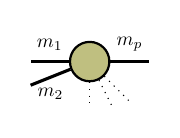
\begin{tikzpicture}[baseline=-0.5ex]
    \tikzset{tensor/.style = {minimum size = 0.5cm,shape = circle,thick,draw=black,inner sep = 0pt}, edge/.style = {thick,line width=.4mm},every loop/.style={}}
    \def\x{6}
    \node[tensor,fill=green!50!red!50!white] (A) at (\x,0) {$\At$};
    \draw[edge] (A) -- (\x-0.75,0) node [midway,above] {\scalebox{0.7}{\dimcolor{$m_1$}}};
    \draw[edge] (A) -- (\x+0.75,0) node [midway,above] {\scalebox{0.7}{\dimcolor{$m_p$}}};;
    \draw[edge] (A) -- (\x-0.75,-0.3) node [midway, below] {\scalebox{0.7}{\dimcolor{$m_2$}}};;
    \draw[dotted] (A) -- (\x,-0.6);
    \draw[dotted] (A) -- (\x+0.5,-0.5);
    \draw[dotted] (A) -- (\x+0.3,-0.6);
    \end{tikzpicture}
\hspace{0.3cm}
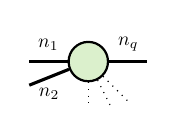
\begin{tikzpicture}[baseline=-0.5ex]
    \tikzset{tensor/.style = {minimum size = 0.5cm,shape = circle,thick,draw=black,inner sep = 0pt}, edge/.style = {thick,line width=.4mm},every loop/.style={}}
    \def\x{6}
    \def\y{0}
    \node[tensor,fill=green!70!red!20!white] (B) at (\x+1,\y) {$\Bt$};
    \draw[edge] (B) -- (\x+0.25,0) node [midway,above] {\scalebox{0.7}{\dimcolor{$n_1$}}};
    \draw[edge] (B) -- (\x+1.75,0) node [midway,above] {\scalebox{0.7}{\dimcolor{$n_q$}}};;
    \draw[edge] (B) -- (\x+0.25,-0.3) node [midway, below] {\scalebox{0.7}{\dimcolor{$n_2$}}};
    \draw[dotted] (B) -- (\x+1,-0.6);
    \draw[dotted] (B) -- (\x+1.5,-0.5);
    \draw[dotted] (B) -- (\x+1.3,-0.6);
\end{tikzpicture}\in\RR^{m_1\times\dots\times m_p\times n_1\times\dots\times n_q}.
$$
More generally, for any arbitrary number of tensors with arbitrary orders, the tensor network diagram of their outer product is obtained by simply placing them next to each other, e.g., for  $\Tt\in\RR^{d_1\times d_2\times d_3 \times d_4}$, $\Ab\in\RR^{m\times n}$ and $\vb\in\RR^{p}$
$$
\Ab\outprod \Tt\outprod \vb
=
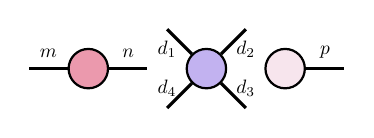
\begin{tikzpicture}[baseline=-0.5ex]
    \tikzset{tensor/.style = {minimum size = 0.5cm,shape = circle,thick,draw=black,inner sep = 0pt}, edge/.style = {thick,line width=.4mm},every loop/.style={}}
    \def\x{0}
    \def\y{0}
    \node[tensor,fill=blue!20!red!40!white] (A) at (\x,\y) {$\Ab$};
    \draw[edge] (A) -- (\x+0.75,\y)node [midway, above] {\scalebox{0.7}{\dimcolor{$n$}}};
    \draw[edge] (A) -- (\x-0.75,\y)node [midway, above] {\scalebox{0.7}{\dimcolor{$m$}}};
    \node[tensor,fill=red!20!blue!30!white] (T) at (\x+1.5,\y) {$\Tt$};
    \node[tensor,fill=red!70!blue!10!white] (v) at (\x+2.5,\y) {$\vb$};
    \draw[edge](T) -- (\x+2,\y-0.5);
    \node[draw=none] () at (\x+2,\y-0.25) {\scalebox{0.7}{\dimcolor{$d_3$}}};
    \draw[edge](T) -- (\x+2,\y+0.5);
    \node[draw=none] () at (\x+2,\y+0.25) {\scalebox{0.7}{\dimcolor{$d_2$}}};
    \draw[edge](T) -- (\x+1,\y-0.5);
    \node[draw=none] () at (\x+1,\y-0.25) {\scalebox{0.7}{\dimcolor{$d_4$}}};
    \draw[edge](T) -- (\x+1,\y+0.5);
    \node[draw=none] () at (\x+1,\y+0.25) {\scalebox{0.7}{\dimcolor{$d_1$}}};
    \draw[edge](v) -- (\x+3.25,\y)node [midway, above] {\scalebox{0.7}{\dimcolor{$p$}}};
\end{tikzpicture}\in\RR^{m\times n \times d_1\times d_2\times d_3 \times d_4\times p},
$$
is defined element-wise by $(\Ab\outprod\Tt\outprod \vb)_{i_1i_2j_1j_2j_3j_4k} = \Ab_{i_1i_2}\Tt_{j_1\cdots j_4}\vb_{k}$, where $i_1\in[m],i_2\in[n],j_l\in[d_l]$ for $l\in[4]$ and $k\in[p]$.

In the proposition below we show a simple visual proof of the fact that inner products of outer products are products of inner products.
\begin{proposition}
    Let $\Xt,\Tt\in\RR^{d_1\times d_2\times\cdots\times d_N}$ with $\Xt = \ab_1\outprod\ab_2\outprod\cdots\outprod\ab_N$ and $\Tt = \tb_1\outprod\tb_2\outprod\cdots\outprod\tb_N$, then $\langle\Xt,\Tt\rangle = \prod_{n=1}^N\langle\ab_n,\tb_n\rangle$.
\begin{proof}
\begin{align*}
\langle\Xt,\Tt\rangle
&=
\left\langle\begin{tikzpicture}[baseline=\baseline]
    \tikzset{tensor/.style = {minimum size = 0.5cm,shape = circle,thick,draw=black,inner sep = 0pt}, edge/.style   = {thick,line width=.4mm}}
    \def\y{0}
     \def\x{0}
\node[tensor,fill=blue!10!white] (a1) at (\x,\y){$\ab_1$};
\node[tensor,fill=blue!10!white](a2) at (\x+1,\y){$\ab_2$};
  \node[tensor,fill=blue!10!white](an) at (\x+3,\y){$\ab_N$};
    \draw[edge] (a1) -- (\x,\y-0.7) node [midway, left] {\scalebox{0.7}{\dimcolor{$d_1$}}};
    \draw[edge] (a2) -- (\x+1,\y-0.7) node [midway, left] {\scalebox{0.7}{\dimcolor{$d_2$}}};
    \draw[edge] (an) -- (\x+3,\y-0.7)  node [midway, left] {\scalebox{0.7}{\dimcolor{$d_N$}}};
    \node (eq) at (\x+2,\y) {$\cdots$};
\end{tikzpicture} \ \scalebox{1.5}{,}
\begin{tikzpicture}[baseline=\baseline]
    \tikzset{tensor/.style = {minimum size = 0.5cm,shape = circle,thick,draw=black,inner sep = 0pt}, edge/.style   = {thick,line width=.4mm}}
    \def\y{0}
     \def\x{0}
\node[tensor,fill=red!10!white] (t1) at (\x,\y){$\tb_1$};
\node[tensor,fill=red!10!white](t2) at (\x+1,\y){$\tb_2$};
  \node[tensor,fill=red!10!white](tn) at (\x+3,\y){$\tb_N$};
    \draw[edge] (t1) -- (\x,\y-0.7) node [midway, left] {\scalebox{0.7}{\dimcolor{$d_1$}}};
    \draw[edge] (t2) -- (\x+1,\y-0.7) node [midway, left] {\scalebox{0.7}{\dimcolor{$d_2$}}};
    \draw[edge] (tn) -- (\x+3,\y-0.7)  node [midway, left] {\scalebox{0.7}{\dimcolor{$d_N$}}};
    \node (eq) at (\x+2,\y) {$\cdots$};
\end{tikzpicture} 
\right\rangle\\
&=
\begin{tikzpicture}[baseline=\baseline]
    \tikzset{tensor/.style = {minimum size = 0.5cm,shape = circle,thick,draw=black,inner sep = 0pt}, edge/.style   = {thick,line width=.4mm}}
    \def\y{0}
     \def\x{0}
\node[tensor,fill=blue!10!white] (a1) at (\x,\y+0.5){$\ab_1$};
\node[tensor,fill=blue!10!white](a2) at (\x+1,\y+0.5){$\ab_2$};
  \node[tensor,fill=blue!10!white](an) at (\x+3,\y+0.5){$\ab_N$};
  \node[tensor,fill=red!10!white] (t1) at (\x,\y-0.5){$\tb_1$};
\node[tensor,fill=red!10!white](t2) at (\x+1,\y-0.5){$\tb_2$};
  \node[tensor,fill=red!10!white](tn) at (\x+3,\y-0.5){$\tb_N$};
    \draw[edge] (a1) -- (t1) node [midway, left] {\scalebox{0.7}{\dimcolor{$d_1$}}};
    \draw[edge] (a2) -- (t2) node [midway, left] {\scalebox{0.7}{\dimcolor{$d_2$}}};
    \draw[edge] (an) -- (tn)  node [midway, left] {\scalebox{0.7}{\dimcolor{$d_N$}}};
    \node (eq) at (\x+2,\y) {$\cdots$};
\end{tikzpicture}
=
\prod_{n=1}^N\langle\ab_n,\tb_n\rangle.
\end{align*}
\end{proof}
\end{proposition}
\paragraph{Edge of dimension one = no edge}
Note that in tensor network diagrams, an edge of size one is equivalent to having no edge. 
For example, in the matrix multiplication, if the contraction edge is of size one, it is equivalent to the outer product of vectors:
\begin{align*}
    \Ab\in\RR^{p\times 1},\ \ \ \Bb\in\RR^{1\times q}, \ \ \ 
(\Ab\Bb)_{ij} 
&=
\begin{tikzpicture}[baseline=\baseline]
   \tikzset{tensor/.style = {minimum size = 0.5cm,shape = circle,thick,draw=black,inner sep = 0pt}, edge/.style = {thick,line width=.4mm},every loop/.style={}}
    \def\y{0}
    \def\x{0}
    \node[tensor,fill=red!50!white] (A) at (\x,\y){\scalebox{0.85}{$\Ab$}};
    \node[tensor,fill=blue!50!white] (B) at (\x+1,\y){\scalebox{0.85}{$\Bb$}};
    \draw[edge] (A) -- (B) node [above,midway] {\scalebox{0.7}{\dimcolor{$1$}}};
    \draw[edge] (\x-0.25,\y) -- (\x-0.75,\y)  node [pos=1.3] {\scalebox{0.7}{\indcolor{$i$}}};
    \draw[edge] (\x+1.25,\y) -- (\x+1.75,\y)  node [pos=1.3] {\scalebox{0.7}{\indcolor{$j$}}};
\end{tikzpicture}\\
&=
\sum_{k=1}^{1}\Ab_{i1}\Bb_{1j}
=
\begin{tikzpicture}[baseline=\baseline]
   \tikzset{tensor/.style = {minimum size = 0.5cm,shape = circle,thick,draw=black,inner sep = 0pt}, edge/.style = {thick,line width=.4mm},every loop/.style={}}
    \def\y{0}
    \def\x{0}
    \node[tensor,fill=red!50!white] (A) at (\x,\y){\scalebox{0.85}{$\ab$}};
    \node[tensor,fill=blue!50!white] (B) at (\x+1,\y){\scalebox{0.85}{$\bb$}};
    \draw[edge] (\x-0.25,\y) -- (\x-0.75,\y)  node[pos=1.3] {\scalebox{0.7}{\indcolor{$i$}}};
    \draw[edge] (\x+1.25,\y) -- (\x+1.75,\y)  node [pos=1.3] {\scalebox{0.7}{\indcolor{$j$}}};
\end{tikzpicture}\\
&=
(\ab\outprod\bb)_{ij},
\end{align*}
where $\ab$ is the unique column of $\Ab$ and $\bb$ the unique row of $\Bb$.
\paragraph{Trace} The trace operation is a special case of tensor contraction applied on square matrices. In tensor networks, the trace is naturally represented by a loop~(self-edge)  connecting the two legs of the matrix:
\begin{align*}
\Ab\in\RR^{d \times d},\hspace{0.5cm}
\tr(\Ab) = \sum_{i=1}^d\Ab_{ii} = \hspace*{-0.5cm}
\begin{tikzpicture}[baseline=\baseline]
   \tikzset{tensor/.style = {minimum size = 0.5cm,shape = circle,thick,draw=black,inner sep = 0pt}, edge/.style = {thick,line width=.4mm},every loop/.style={}}
    \def\y{0}
    \def\x{0}
    \node[tensor,fill=red!50!white] (A) at (\x,\y){\scalebox{0.85}{$\Ab$}};
    \draw[edge] (A) to [out=20,in=160, distance=1cm] (A);
    \node[draw=none] () at (\x,\y+0.5) {\scalebox{0.7}{\dimcolor{$d$}}};
    \end{tikzpicture}\hspace*{-0.5cm}.
\end{align*}
Since there are no free legs, it is consistent with the fact that the trace is a scalar. Tensor network diagrams offer a very simple proof of the invariance of the trace under cyclic permutation. Let's start with the trace of the product of two matrices $\Ab \in \RR^{d\times R}$ and $\Bb \in \RR^{R\times d}$.  As we explained before, when drawing the graph of a tensor network, only the graph structure is important. This allows us to see that
\begin{align*}
\tr(\Ab\Bb)= 
\hspace{-0.5cm}
\begin{tikzpicture}[baseline=\baseline]
   \tikzset{tensor/.style = {minimum size = 0.5cm,shape = circle,thick,draw=black,inner sep = 0pt}, edge/.style = {thick,line width=.4mm},every loop/.style={}}
    \def\y{0}
    \def\x{0}
    \node[tensor,fill=red!50!white] (A) at (\x,\y){\scalebox{0.85}{$\Ab$}};
    \node[tensor,fill=blue!50!white] (B) at (\x+1,\y){\scalebox{0.85}{$\Bb$}};
    \draw[edge] (A) -- (B) node [midway,above]{\scalebox{0.7}{\dimcolor{$R$}}};
    \draw[edge] (A) to [out=155,in=25, distance=1cm] (B);
    \node[draw=none] () at (\x+0.5,\y+0.65) {\scalebox{0.7}{\dimcolor{$d$}}};
    \end{tikzpicture}
\hspace{-0.5cm} = 
\begin{tikzpicture}[baseline=\baseline]
   \tikzset{tensor/.style = {minimum size = 0.5cm,shape = circle,thick,draw=black,inner sep = 0pt}, edge/.style = {thick,line width=.4mm},every loop/.style={}}
    \def\y{0}
    \def\x{0}
    \node[tensor,fill=red!50!white] (A) at (\x,\y-0.5){\scalebox{0.85}{$\Ab$}};
    \node[tensor,fill=blue!50!white] (B) at (\x,\y+0.5){\scalebox{0.85}{$\Bb$}};
    \draw[edge] (A) to [out=180,in=180, distance=0.5cm] (B);
    \draw[edge] (A) to [out=0,in=0, distance=0.5cm] (B);
    \node[draw=none] () at (\x+0.8,\y) {\scalebox{0.7}{\dimcolor{$R$}}};
    \node[draw=none] () at (\x-0.8,\y) {\scalebox{0.7}{\dimcolor{$d$}}};
    \end{tikzpicture}
 =\hspace{-0.5cm}
\begin{tikzpicture}[baseline=\baseline]
   \tikzset{tensor/.style = {minimum size = 0.5cm,shape = circle,thick,draw=black,inner sep = 0pt}, edge/.style = {thick,line width=.4mm},every loop/.style={}}
    \def\y{0}
    \def\x{0}
    \node[tensor,fill=blue!50!white] (B) at (\x,\y){\scalebox{0.85}{$\Bb$}};
    \node[tensor,fill=red!50!white] (A) at (\x+1,\y){\scalebox{0.85}{$\Ab$}};
    \draw[edge] (A) -- (B)node [midway,above]{\scalebox{0.7}{\dimcolor{$R$}}};;
    \draw[edge] (B) to [out=155,in=25, distance=1cm] (A);
    \node[draw=none] () at (\x+0.5,\y+0.65) {\scalebox{0.7}{\dimcolor{$d$}}};
    \end{tikzpicture}
\hspace{-0.4cm} =
\tr(\Bb\Ab),
\end{align*}
and similarly for three matrices $\Ab\in\RR^{m\times n}, \Bb\in\RR^{n\times p},  \Cb\in\RR^{p\times m}$, we have
\begin{align*}
\tr(\Ab\Bb\Cb) = 
\hspace{-0.7cm}
\begin{tikzpicture}[baseline=\baseline]
   \tikzset{tensor/.style = {minimum size = 0.5cm,shape = circle,thick,draw=black,inner sep = 0pt}, edge/.style = {thick,line width=.4mm},every loop/.style={}}
    \def\y{0}
    \def\x{0}
    \node[tensor,fill=red!50!white] (A) at (\x,\y){\scalebox{0.85}{$\Ab$}};
    \node[tensor,fill=blue!50!white] (B) at (\x+1,\y){\scalebox{0.85}{$\Bb$}};
    \node[tensor,fill=red!30!white] (C) at (\x+2,\y){\scalebox{0.85}{$\Cb$}};
    \draw[edge] (A) -- (B) node [midway,above]{\scalebox{0.7}{\dimcolor{$n$}}};
    \draw[edge] (B) -- (C) node [midway,above]{\scalebox{0.7}{\dimcolor{$p$}}};;
    \draw[edge] (A) to [out=155,in=25, distance=1cm] (C);
    \node[draw=none] () at (\x+1,\y+0.65) {\scalebox{0.7}{\dimcolor{$m$}}};
    \end{tikzpicture}
\hspace{-0.7cm}  = 
\begin{tikzpicture}[baseline=\baseline]
   \tikzset{tensor/.style = {minimum size = 0.5cm,shape = circle,thick,draw=black,inner sep = 0pt}, edge/.style = {thick,line width=.4mm},every loop/.style={}}
    \def\y{0}
    \def\x{0}
    \node[tensor,fill=red!50!white] (A) at (\x,\y+0.5){\scalebox{0.85}{$\Ab$}};
    \node[tensor,fill=blue!50!white] (B) at (\x-0.5,\y-0.3){\scalebox{0.85}{$\Bb$}};
    \node[tensor,fill=red!30!white] (C) at (\x+0.5,\y-0.3){\scalebox{0.85}{$\Cb$}};
    \draw[edge] (A) to [out=210,in=90] (B);
    \draw[edge] (A) to [out=-30,in=90] (C);
    \draw[edge] (B) to [out=300,in=240] (C);
    \node[draw=none] () at (\x+0.55,\y+0.3) {\scalebox{0.7}{\dimcolor{$m$}}};
    \node[draw=none] () at (\x-0.55,\y+0.3) {\scalebox{0.7}{\dimcolor{$n$}}};
    \node[draw=none] () at (\x,\y-0.85) {\scalebox{0.7}{\dimcolor{$p$}}};
    \end{tikzpicture}
= 
\hspace{-0.7cm}
\begin{tikzpicture}[baseline=\baseline]
   \tikzset{tensor/.style = {minimum size = 0.5cm,shape = circle,thick,draw=black,inner sep = 0pt}, edge/.style = {thick,line width=.4mm},every loop/.style={}}
    \def\y{0}
    \def\x{0}
    \node[tensor,fill=red!30!white] (C) at (\x,\y){\scalebox{0.85}{$\Cb$}};
    \node[tensor,fill=red!50!white] (A) at (\x+1,\y){\scalebox{0.85}{$\Ab$}};
    \node[tensor,fill=blue!50!white] (B) at (\x+2,\y){\scalebox{0.85}{$\Bb$}};
    \draw[edge] (C) -- (A) node [midway,above]{\scalebox{0.7}{\dimcolor{$m$}}};
    \draw[edge] (A) -- (B) node [midway,above]{\scalebox{0.7}{\dimcolor{$n$}}};
    \draw[edge] (C) to [out=155,in=25, distance=1cm] (B);
    \node[draw=none] () at (\x+1,\y+0.65) {\scalebox{0.7}{\dimcolor{$p$}}};
    \end{tikzpicture}
\hspace{-0.7cm} = \tr(\Cb\Ab\Bb).
\end{align*}
Note that the equalities between the  tensor network diagrams are trivial: we just changed the nodes' position without changing the underlying graph's structure. We thus simply interpreted the same diagram in two ways, leading to a less trivial equality between $\tr(\Ab\Bb\Cb)$ and $\tr(\Cb\Ab\Bb)$.

\paragraph{Partial traces} The \emph{partial trace} is a common operation used in particular in the context of modeling many-body quantum systems, where density matrices of a part of a system are obtained by performing a partial trace of the density matrix of the whole system. Without delving into the specifics of quantum systems, consider a square matrix  of dimension $d_1d_2\times d_1d_2$ which we interpret as a fourth-order tensor \begin{tikzpicture}[baseline=-0.5ex]
    \tikzset{tensor/.style = {minimum width = 0.8cm,minimum height = 0.4cm,shape = rounded rectangle,thick,draw=black,inner sep = 0pt}, edge/.style = {thick,line width=.4mm},every loop/.style={}}
    \def\x{0}
    \def\y{0}
    \draw[edge] (\x-0.2,\y-0.15) -- (\x-0.2,\y-0.5)node [midway,left=-0.05cm] {\scalebox{0.7}{\dimcolor{$d_1$}}};
    \draw[edge] (\x+0.2,\y-0.15) -- (\x+0.2,\y-0.5)node [midway,right=-0.05cm] {\scalebox{0.7}{\dimcolor{$d_2$}}};
    \draw[edge] (\x-0.2,\y+0.15) -- (\x-0.2,\y+0.5)node [midway,left=-0.05cm] {\scalebox{0.7}{\dimcolor{$d_1$}}};
    \draw[edge] (\x+0.2,\y+0.15) -- (\x+0.2,\y+0.5)node [midway,right=-0.05cm] {\scalebox{0.7}{\dimcolor{$d_2$}}};
    \node[tensor,fill=yellow] (Bt) at (\x,\y){$\Tt$};
    \end{tikzpicture}.
The partial trace of $\Tt$ over the subspace $\mathbb R^{d_1}$ is the $d_2\times d_2$ matrix obtained by ``tracing out'' the $d_1$ dimension by connecting the corresponding legs: \begin{tikzpicture}[baseline=-0.5ex]
    \tikzset{tensor/.style = {minimum width = 0.6cm,minimum height = 0.4cm,shape = rounded rectangle,thick,draw=black,inner sep = 0pt}, edge/.style = {thick,line width=.4mm},every loop/.style={}}
    \def\x{0}
    \def\y{0}
    \draw[edge] (\x-0.2,\y-0.15) -- (\x-0.2,\y-0.4);
    \draw[edge] (\x+0.2,\y-0.15) -- (\x+0.2,\y-0.5)node [midway,right=-0.05cm] {\scalebox{0.7}{\dimcolor{$d_2$}}};
    \draw[edge] (\x-0.2,\y+0.15) -- (\x-0.2,\y+0.4);
    \draw[edge] (\x+0.2,\y+0.15) -- (\x+0.2,\y+0.5)node [midway,right=-0.05cm] {\scalebox{0.7}{\dimcolor{$d_2$}}};
    \draw[edge] (\x-0.2,\y-0.39) to [out=200,in=160] (\x-0.2,\y+0.39) node [midway,left=0.35cm] {\scalebox{0.7}{\dimcolor{$d_1$}}};
    \node[tensor,fill=yellow] (Bt) at (\x,\y){$\Tt$};
    \end{tikzpicture}. Similarly, the partial trace of $\Tt$ over the subspace $\mathbb R^{d_2}$ is the $d_1\times d_1$ matrix 
\begin{tikzpicture}[baseline=-0.5ex]
    \tikzset{tensor/.style = {minimum width = 0.6cm,minimum height = 0.4cm,shape = rounded rectangle,thick,draw=black,inner sep = 0pt}, edge/.style = {thick,line width=.4mm},every loop/.style={}}
    \def\x{0}
    \def\y{0}
    \draw[edge] (\x-0.2,\y-0.15) -- (\x-0.2,\y-0.5)node [midway,left=-0.05cm] {\scalebox{0.7}{\dimcolor{$d_1$}}};
    \draw[edge] (\x+0.2,\y-0.15) -- (\x+0.2,\y-0.4);
    \draw[edge] (\x-0.2,\y+0.15) -- (\x-0.2,\y+0.5)node [midway,left=-0.05cm] {\scalebox{0.7}{\dimcolor{$d_1$}}};
    \draw[edge] (\x+0.2,\y+0.15) -- (\x+0.2,\y+0.4);
    \draw[edge] (\x+0.2,\y-0.39) to [out=330,in=30] (\x+0.2,\y+0.39) node [midway,right=0.3cm] {\scalebox{0.7}{\dimcolor{$d_2$}}};
    \node[tensor,fill=yellow] (Bt) at (\x,\y){$\Tt$};
\end{tikzpicture}.

\paragraph{Tensor Frobenius Norm} The Frobenius norm of a tensor $\At\in\RR^{d_1\times\cdots\times d_N}$ is the square root of the sum of its
squared elements~(i.e., the square root of the inner product with itself). In tensor networks, the norm of a third-order tensor $\At\in\RR^{d_1\times d_2\times d_3}$ is represented as
\begin{align*}
\norm{\At}_F^2 = \langle\At,\At\rangle = 
\sum_{i_1=1}^{d_1}\sum_{i_2=1}^{d_2}\sum_{i_3=1}^{d_3}\At_{i_1i_2i_3}^2
=
\begin{tikzpicture}[baseline=\baseline]
    \tikzset{tensor/.style = {minimum size = 0.5cm,shape = circle,thick,draw=black,inner sep = 0pt}, edge/.style = {thick,line width=.4mm},every loop/.style={}}
    \def\y{0}
    \def\x{0}
    \node[tensor,fill=green!50!red!50!white] (At) at (\x,\y){\scalebox{0.85}{$\At$}};
    \node[tensor,fill=green!50!red!50!white] (At1) at (\x+1,\y){\scalebox{0.85}{$\At$}};
    \draw[edge] (At) -- (At1);
    \draw[edge] (At) to [out=45,in=135] (At1);
    \draw[edge] (At) to [out=-45,in=-135] (At1);
    \node[draw=none] () at (\x+0.5,\y+0.6) {\scalebox{0.7}{\dimcolor{$d_1$}}};
    \node[draw=none] () at (\x+0.5,\y+0.15) {\scalebox{0.7}{\dimcolor{$d_2$}}};
    \node[draw=none] () at (\x+0.5,\y-0.5) {\scalebox{0.7}{\dimcolor{$d_3$}}};
\end{tikzpicture} .
\end{align*}
It is a direct and natural generalization of the matrix Frobenius norm: 
\begin{align*}
 \norm{\Ab}_F^2 = \tr(\Ab\Ab^\ts) = \tr(\Ab^\ts\Ab) =  \hspace*{-0.5cm}
\begin{tikzpicture}[baseline=\baseline]
   \tikzset{tensor/.style = {minimum size = 0.5cm,shape = circle,thick,draw=black,inner sep = 0pt}, edge/.style = {thick,line width=.4mm},every loop/.style={}}
    \def\y{0}
    \def\x{0}
    \node[tensor,fill=red!50!white] (A) at (\x,\y){\scalebox{0.85}{$\Ab$}};
    \node[tensor,fill=red!50!white] (B) at (\x+1,\y){\scalebox{0.85}{$\Ab$}};
    \draw[edge] (A) -- (B) node [midway,above]{\scalebox{0.7}{\dimcolor{$n$}}};
    \draw[edge] (A) to [out=155,in=25, distance=1cm] (B);
    \node[draw=none] () at (\x+0.5,\y+0.65) {\scalebox{0.7}{\dimcolor{$m$}}};
    \end{tikzpicture} \hspace*{-0.5cm}.
\end{align*}


\paragraph{Frobenius norm of outer products} Using tensor networks, it is almost trivial to show that the Frobenius norm of an outer product is equal to the product of the Frobenius norms. E.g., for $\Ab\in\RR^{m\times n}$ and $\Tt\in\RR^{d_1\times d_2\times d_3}$, we have 
$$ \begin{tikzpicture}[baseline=-0.5ex]
    \tikzset{tensor/.style = {minimum width = 1.8cm,minimum height = 0.4cm,shape = rounded rectangle,thick,draw=black,inner sep = 0pt}, edge/.style = {thick,line width=.4mm},every loop/.style={}}
    \def\x{0}
    \def\y{0}
    \draw[edge] (\x-0.7,\y-0.15) -- (\x-0.7,\y-0.5)node [midway,left=-0.05cm] {\scalebox{0.7}{\dimcolor{$m$}}};
    \draw[edge] (\x-0.35,\y-0.15) -- (\x-0.35,\y-0.5)node [midway,left=-0.05cm] {\scalebox{0.7}{\dimcolor{$n$}}};
    \draw[edge] (\x,\y-0.15) -- (\x,\y-0.5)node [midway,left=-0.1cm] {\scalebox{0.7}{\dimcolor{$d_1$}}};
    \draw[edge] (\x+0.35,\y-0.15) -- (\x+0.35,\y-0.5)node [midway,left=-0.1cm] {\scalebox{0.7}{\dimcolor{$d_2$}}};
    \draw[edge] (\x+0.7,\y-0.15) -- (\x+0.7,\y-0.5)node [midway,left=-0.1cm] {\scalebox{0.7}{\dimcolor{$d_3$}}};
    \node[tensor,fill=yellow] (Bt) at (\x,\y){$\Ab \outprod \Tt$};
    \end{tikzpicture}
    = 
    \begin{tikzpicture}[baseline=\baseline]
   \tikzset{tensor/.style = {minimum width = 0.8cm,minimum height = 0.4cm,shape = rounded rectangle,thick,draw=black,inner sep = 0pt}, edge/.style = {thick,line width=.4mm},every loop/.style={}}
    \def\y{0}
    \def\x{0}
    \draw[edge] (\x+0.2,\y-0.15) -- (\x+0.2,\y-0.5) node [midway,left=-0.05cm]{\scalebox{0.7}{\dimcolor{$n$}}};
    \draw[edge] (\x-0.2,\y-0.15) -- (\x-0.2,\y-0.5) node [midway,left=-0.05cm]{\scalebox{0.7}{\dimcolor{$m$}}};
    \node[tensor,fill=red!50!white] (A) at (\x,\y){{$\Ab$}};

   
    \def\y{0}
    \def\x{1}
    \draw[edge] (\x-0.3,\y-0.15) -- (\x-0.3,\y-0.5) node [midway,left=-0.1cm]{\scalebox{0.7}{\dimcolor{$d_1$}}};
    \draw[edge] (\x+0.05,\y-0.15) -- (\x+0.05,\y-0.5) node [midway,left=-0.1cm]{\scalebox{0.7}{\dimcolor{$d_2$}}};
    \draw[edge] (\x+0.3,\y-0.15) -- (\x+0.3,\y-0.5) node [midway,right=-0.05cm]{\scalebox{0.7}{\dimcolor{$d_3$}}};
    \node[tensor,fill=red!30!blue!20!white] (T) at (\x,\y){{$\Tt$}};
\end{tikzpicture}
    $$
and thus
\begin{align*}
\norm{\Ab\outprod\Tt}_F^2
=
\norm{
\begin{tikzpicture}[baseline=\baseline]
\tikzset{tensor/.style = {minimum width = 1.8cm,minimum height = 0.4cm,shape = rounded rectangle,thick,draw=black,inner sep = 0pt}, edge/.style = {thick,line width=.4mm},every loop/.style={}}
    \def\x{0}
    \def\y{0}
    \draw[edge] (\x-0.7,\y-0.15) -- (\x-0.7,\y-0.5)node [midway,left=-0.05cm] {\scalebox{0.7}{\dimcolor{$m$}}};
    \draw[edge] (\x-0.35,\y-0.15) -- (\x-0.35,\y-0.5)node [midway,left=-0.05cm] {\scalebox{0.7}{\dimcolor{$n$}}};
    \draw[edge] (\x,\y-0.15) -- (\x,\y-0.5)node [midway,left=-0.1cm] {\scalebox{0.7}{\dimcolor{$d_1$}}};
    \draw[edge] (\x+0.35,\y-0.15) -- (\x+0.35,\y-0.5)node [midway,left=-0.1cm] {\scalebox{0.7}{\dimcolor{$d_2$}}};
    \draw[edge] (\x+0.7,\y-0.15) -- (\x+0.7,\y-0.5)node [midway,left=-0.1cm] {\scalebox{0.7}{\dimcolor{$d_3$}}};
    \node[tensor,fill=yellow] (Bt) at (\x,\y){$\Ab \outprod \Tt$};
\end{tikzpicture}
}_F^2
=
\begin{tikzpicture}[baseline=\baseline]
\tikzset{tensor/.style = {minimum width = 1.8cm,minimum height = 0.4cm,shape = rounded rectangle,thick,draw=black,inner sep = 0pt}, edge/.style = {thick,line width=.4mm},every loop/.style={}}
    \def\x{0}
    \def\y{0.35}
    \draw[edge] (\x-0.7,\y-0.15) -- (\x-0.7,\y-0.5)node [midway,left=-0.05cm] {\scalebox{0.7}{\dimcolor{$m$}}};
    \draw[edge] (\x-0.35,\y-0.15) -- (\x-0.35,\y-0.5)node [midway,left=-0.05cm] {\scalebox{0.7}{\dimcolor{$n$}}};
    \draw[edge] (\x,\y-0.15) -- (\x,\y-0.5)node [midway,left=-0.1cm] {\scalebox{0.7}{\dimcolor{$d_1$}}};
    \draw[edge] (\x+0.35,\y-0.15) -- (\x+0.35,\y-0.5)node [midway,left=-0.1cm] {\scalebox{0.7}{\dimcolor{$d_2$}}};
    \draw[edge] (\x+0.7,\y-0.15) -- (\x+0.7,\y-0.5)node [midway,left=-0.1cm] {\scalebox{0.7}{\dimcolor{$d_3$}}};
    \node[tensor,fill=yellow] (Bt) at (\x,\y){$\Ab \outprod \Tt$};
    \node[tensor,fill=yellow] (Bt) at (\x,\y-0.7){$\Ab \outprod \Tt$};
\end{tikzpicture}
=
\begin{tikzpicture}[baseline=\baseline]
   \tikzset{tensor/.style = {minimum width = 0.9cm,minimum height = 0.4cm,shape = rounded rectangle,thick,draw=black,inner sep = 0pt}, edge/.style = {thick,line width=.4mm},every loop/.style={}}
    \def\y{0.35}
    \def\x{0}
    \draw[edge] (\x+0.2,\y-0.15) -- (\x+0.2,\y-0.5) node [midway,left=-0.05cm]{\scalebox{0.7}{\dimcolor{$n$}}};
    \draw[edge] (\x-0.2,\y-0.15) -- (\x-0.2,\y-0.5) node [midway,left=-0.05cm]{\scalebox{0.7}{\dimcolor{$m$}}};
    \node[tensor,fill=red!50!white] (A) at (\x,\y){{$\Ab$}};
    \node[tensor,fill=red!50!white] (A) at (\x,\y-0.7){{$\Ab$}};
    \def\x{1}
    \draw[edge] (\x-0.3,\y-0.15) -- (\x-0.3,\y-0.5) node [midway,left=-0.1cm]{\scalebox{0.7}{\dimcolor{$d_1$}}};
    \draw[edge] (\x+0.05,\y-0.15) -- (\x+0.05,\y-0.5) node [midway,left=-0.1cm]{\scalebox{0.7}{\dimcolor{$d_2$}}};
    \draw[edge] (\x+0.3,\y-0.15) -- (\x+0.3,\y-0.5) node [midway,right=-0.1cm]{\scalebox{0.7}{\dimcolor{$d_3$}}};
    \node[tensor,fill=red!30!blue!20!white] (T) at (\x,\y){{$\Tt$}};
    \node[tensor,fill=red!30!blue!20!white] (T) at (\x,\y-0.7){{$\Tt$}};
\end{tikzpicture}
=\norm{\Ab}_F^2 \norm{\Tt}_F^2
.
\end{align*}


\paragraph{Example} We conclude this section with a last example showing how the tensor network graphical notation is very useful for representing complicated operations on tensors:
\begin{align}\label{eq:einsum}
\begin{tikzpicture}[baseline = \baseline]
    \tikzset{tensor/.style = {minimum size = 0.5cm,shape = circle,thick,draw=black,inner sep = 0pt}, edge/.style = 
    {thick,line width=.4mm},every loop/.style={}}
    \def\y{-0.5}
    \def\x{0}
    \node[tensor,fill=green!50!red!50!white] (At) at (\x,\y){\scalebox{0.85}{$\At$}};
    \node[tensor,fill=red!20!white] (S) at (\x-1,\y){\scalebox{0.85}{$\St$}};
    \node[tensor,fill=red!50!white] (Tt) at (\x,\y+1){\scalebox{0.85}{$\Tt$}};
    \node[tensor,fill=blue!40!red!60!white] (A) at (\x+1,\y){\scalebox{0.85}{$\Ab$}};
    \draw[edge] (Tt) -- (At) node [midway,left] {\scalebox{0.7}{\dimcolor{$R$}}};
    \draw[edge] (Tt) -- (A) node [above,midway] {\scalebox{0.7}{\dimcolor{$R$}}};
    \draw[edge] (At) -- (A)  node [midway,above] {\scalebox{0.7}{\dimcolor{$R$}}};
    \draw[edge] (Tt) -- (\x,\y+1.75) node [pos=1.3] {\scalebox{0.7}{\indcolor{$k$}}};
    \draw[edge] (At) -- (S)  node [midway,above] {\scalebox{0.7}{\dimcolor{$R$}}};
    \draw[edge] (S) -- (Tt)  node [midway,above] {\scalebox{0.7}{\dimcolor{$R$}}};
    \draw[edge] (Tt) -- (\x-0.75,\y+1)  node [pos=1.3] {\scalebox{0.7}{\indcolor{$j$}}};
    \draw[edge] (Tt) -- (\x+0.75,\y+1)  node [pos=1.3] {\scalebox{0.7}{\indcolor{$l$}}};
    \draw[edge] (S) -- (\x-1.2,\y+0.75)  node [pos=1.3] {\scalebox{0.7}{\indcolor{$i$}}};
    \end{tikzpicture}
&=
\sum_{r_1=1}^R\sum_{r_2=1}^R\sum_{r_3=1}^R\sum_{r_4=1}^R\sum_{r_5=1}^R\St_{ir_1 r_2}\At_{r_2r_3r_5}\Tt_{iklr_1r_3r_4}\Ab_{r_4r_5}\nonumber\\
&=
    \begin{tikzpicture}[baseline = \baseline]
    \tikzset{tensor/.style = {minimum size = 0.5cm,shape = circle,thick,draw=black,inner sep = 0pt}, edge/.style = 
    {thick,line width=.4mm},every loop/.style={}}
    \def\y{0}
    \def\x{0}
    \node[tensor,fill=blue!50!red!30!yellow!50!white] (Ht) at (\x,\y){\scalebox{0.85}{$\Ht$}};
    \draw[edge](Ht) -- (\x,\y+0.7) node [pos=1.3] {\scalebox{0.7}{\indcolor{$j$}}};
    \draw[edge](Ht) -- (\x,\y-0.7) node [pos=1.3] {\scalebox{0.7}{\indcolor{$l$}}};
    \draw[edge](Ht) -- (\x-0.7,\y) node [pos=1.3] {\scalebox{0.7}{\indcolor{$i$}}};
    \draw[edge](Ht) -- (\x+0.7,\y) node[pos=1.3] {\scalebox{0.7}{\indcolor{$k$}}};
    \end{tikzpicture}.
\end{align}
\subsection{Copy Tensors~(Hyperedges)}\label{sec:copy-tensor}


Sometimes, one needs to represent a simultaneous contraction shared among more than two tensors. Consider, for example, the following contraction between three vectors, $\ab\in\RR^d, \bb\in\RR^d,$ and $\cbb\in\RR^d$ to obtain a scalar: $\sum_{i=1}^d\ab_i\bb_i\cbb_i$.
This operation can be depicted in tensor networks using a special tensor called \emph{copy tensor}. The copy tensor is equivalent to a Kronecker delta, i.e., a hyper-diagonal tensor with ones on the diagonal and zeros elsewhere, and is represented as a black dot in tensor network diagrams. E.g., the copy tensor  
\begin{tikzpicture}[baseline=\baseline]
   \tikzset{tensor/.style = {minimum size = 0.5cm,shape = circle,thick,draw=black,inner sep = 0pt}, edge/.style = {thick,line width=.4mm},every loop/.style={}}
    \def\y{0}
    \def\x{0}
     \draw  node[fill = black,circle,inner sep=0pt,minimum size=4pt] (m) at (\x,\y) {};
     \draw  node[draw=none] (a) at (\x-0.7,\y) {};
     \draw  node[draw=none] (b) at (\x+0.7,\y) {};
     \draw  node[draw=none] (c) at (\x,\y-0.7) {};
    \draw[edge] (a) -- (m);
    \draw[edge] (m) -- (b);
    \draw[edge] (m) -- (c);
\end{tikzpicture}
is defined element-wise as
$$
 \left(\begin{tikzpicture}[baseline=\baseline]
   \tikzset{tensor/.style = {minimum size = 0.5cm,shape = circle,thick,draw=black,inner sep = 0pt}, edge/.style = {thick,line width=.4mm},every loop/.style={}}
    \def\y{0}
    \def\x{0}
     \draw  node[fill = black,circle,inner sep=0pt,minimum size=4pt] (m) at (\x,\y) {};
     \draw  node[draw=none] (a) at (\x-0.7,\y) {};
     \draw  node[draw=none] (b) at (\x+0.7,\y) {};
     \draw  node[draw=none] (c) at (\x,\y-0.7) {};
    \draw[edge] (a) -- (m);
    \draw[edge] (m) -- (b);
    \draw[edge] (m) -- (c);
\end{tikzpicture}\right)_{ijk} = \delta_{ijk} = \begin{cases}
      1 & \text{if } i=j=k\\
      0 & \text{otherwise}
    \end{cases}.
$$
Using the copy tensor, the 3-way contraction mentioned above can be represented as 
\begin{align*}
\begin{tikzpicture}[baseline=\baseline]
   \tikzset{tensor/.style = {minimum size = 0.5cm,shape = circle,thick,draw=black,inner sep = 0pt}, edge/.style = {thick,line width=.4mm},every loop/.style={}}
    \def\y{0}
    \def\x{0}
    \node[tensor,fill=blue!40!red!60!white] (a) at (\x,\y){\scalebox{0.85}{$\ab$}};
    \node[tensor,fill=blue!10!white] (b) at (\x+1.5,\y){\scalebox{0.85}{$\bb$}};
    \node[tensor,fill=blue!20!red!40!white] (c) at (\x+0.7,\y-0.75){\scalebox{0.85}{$\cbb$}};
    \draw  node[fill = black,circle,inner sep=0pt,minimum size=4pt] (m) at (\x+0.7,\y) {};
    \draw[edge] (a) -- (m) node [above,midway] {\scalebox{0.7}{\dimcolor{$d$}}};
    \draw[edge] (m) -- (b) node [above,midway] {\scalebox{0.7}{\dimcolor{$d$}}};
    \draw[edge] (m) -- (c) node [left,midway] {\scalebox{0.7}{\dimcolor{$d$}}};
    \end{tikzpicture} = \sum_{i,j,k=1}^d\delta_{ijk}\ab_i\bb_j\cbb_k =
\sum_{i=1}^d\ab_i\bb_i\cbb_i .
\end{align*}
We now give a more formal definition of the copy tensor of arbitrary order $N$.
\begin{definition}
N-th order copy tensor
   \begin{tikzpicture}[baseline=\baseline]
    \tikzset{tensor/.style = {minimum size = 0.5cm,shape = circle,thick,draw=black,inner sep = 0pt}, edge/.style   = {thick,line width=.4mm},every loop/.style={}}
    \def\y{0}
    \def\x{0}
    \draw  node[fill = black,circle,inner sep=0pt,minimum size=4pt] (m) at (\x,\y) {};
    \draw[edge] (m) -- (\x-0.6,0) node [midway,above] {\scalebox{0.7}{\dimcolor{$d$}}};
    \draw[edge] (m) -- (\x+0.6,0) node [midway,above] {\scalebox{0.7}{\dimcolor{$d$}}};;
    \draw[edge] (m) -- (\x-0.5,-0.3) node [midway, below] {\scalebox{0.7}{\dimcolor{$d$}}};;
    \draw[dotted] (m) -- (\x,-0.6);
    \draw[dotted] (m) -- (\x,-0.6);
    \draw[dotted] (m) -- (\x+0.5,-0.5);
    \draw[dotted] (m) -- (\x+0.3,-0.6);
\end{tikzpicture}
is the tensor of shape $\underbrace{d\times d\dots\times d}_{N\text{ times}}$ defined by 
\begin{align*}
       \begin{tikzpicture}[baseline=\baseline]
    \tikzset{tensor/.style = {minimum size = 0.5cm,shape = circle,thick,draw=black,inner sep = 0pt}, edge/.style   = {thick,line width=.4mm},every loop/.style={}}
    \def\y{0}
    \def\x{0}
    \draw  node[fill = black,circle,inner sep=0pt,minimum size=4pt] (m) at (\x,\y) {};
    \draw[edge] (m) -- (\x-0.6,0) node [midway,above] {\scalebox{0.7}{\dimcolor{$d$}}};
    \draw[edge] (m) -- (\x+0.6,0) node [midway,above] {\scalebox{0.7}{\dimcolor{$d$}}};;
    \draw[edge] (m) -- (\x-0.5,-0.3) node [midway, below] {\scalebox{0.7}{\dimcolor{$d$}}};;
    \draw[dotted] (m) -- (\x,-0.6);
    \draw[dotted] (m) -- (\x,-0.6);
    \draw[dotted] (m) -- (\x+0.5,-0.5);
    \draw[dotted] (m) -- (\x+0.3,-0.6);
\end{tikzpicture}
= \sum_{i=1}^d\underbrace{\eb_i\outprod\eb_i\outprod\dots\outprod\eb_i}_{N\text{ times}},%
\end{align*}
where $\eb_1,\eb_2,\dots,\eb_d$ are the vectors of the canonical basis of $\RR^{d}$.
\end{definition}
The name copy tensor comes from the fact that one can "copy" the canonical vectors by contraction with the copy tensor. Indeed, let $\eb_i\in\RR^{d}$ be a canonical basis vector, then one 
can check that
$       
\begin{tikzpicture}[baseline=\baseline]
    \tikzset{tensor/.style = {minimum size = 0.5cm,shape = circle,thick,draw=black,inner sep = 0pt}, edge/.style   = {thick,line width=.4mm},every loop/.style={}}
    \def\y{0}
    \def\x{0}
    \node[tensor,fill=blue!40!red!60!white] (e) at (\x,\y){\scalebox{0.85}{$\eb_i$}};
    \draw  node[fill = black,circle,inner sep=0pt,minimum size=4pt] (m) at (\x+0.75,\y) {};
    \draw[edge] (e) -- (m) node [midway,above] {\scalebox{0.7}{\dimcolor{$d$}}};
    \draw[edge] (m) -- (\x+1.4,\y) node [midway,above] {\scalebox{0.7}{\dimcolor{$d$}}};
    \draw[edge] (m) -- (\x+0.75,\y-0.7) node [midway,right] {\scalebox{0.7}{\dimcolor{$d$}}};
    \node[draw=none] () at (\x+2,\y) {\scalebox{1}{$=$}};
    \node[tensor,fill=blue!40!red!60!white] (e1) at (\x+2.5,\y){\scalebox{0.85}{$\eb_i$}};
    \node[tensor,fill=blue!40!red!60!white] (e2) at (\x+3.5,\y){\scalebox{0.85}{$\eb_i$}};
    \draw[edge] (e2) -- (\x+3.5,\y-0.7) node [midway,right] {\scalebox{0.7}{\textcolor{gray}{$d$}}};
    \draw[edge] (e1) -- (\x+2.5,\y-0.7) node [midway,right] {\scalebox{0.7}{\textcolor{gray}{$d$}}};
\end{tikzpicture}.
$
Here is a short proof of this fact:
\begin{align*}
    \left(
\begin{tikzpicture}[baseline=\baseline]
    \tikzset{tensor/.style = {minimum size = 0.5cm,shape = circle,thick,draw=black,inner sep = 0pt}, edge/.style   = {thick,line width=.4mm},every loop/.style={}}
    \def\y{0}
    \def\x{0}
    \node[tensor,fill=blue!40!red!60!white] (e) at (\x,\y){\scalebox{0.85}{$\eb_i$}};
    \draw  node[fill = black,circle,inner sep=0pt,minimum size=4pt] (m) at (\x+0.75,\y) {};
    \draw[edge] (e) -- (m) node [midway,above] {\scalebox{0.7}{\dimcolor{$d$}}};
    \draw[edge] (m) -- (\x+1.4,\y) node [midway,above] {\scalebox{0.7}{\dimcolor{$d$}}};
    \draw[edge] (m) -- (\x+0.75,\y-0.7)node [midway,right] {\scalebox{0.7}{\dimcolor{$d$}}};
\end{tikzpicture}\right)_{jk}
&= 
\sum_{s}(\eb_i)_{s}\delta_{sjk} = \sum_{s}\delta_{is}\delta_{sjk} = \delta_{ijk}\\ 
&= 
\begin{cases}
     1 & \text{if } i=j=k\\
      0 & \text{otherwise}.
    \end{cases} =
    (\eb_i\eb_i^\ts)_{j,k} =
\begin{tikzpicture}[baseline=\baseline]
    \tikzset{tensor/.style = {minimum size = 0.5cm,shape = circle,thick,draw=black,inner sep = 0pt}, edge/.style   = {thick,line width=.4mm},every loop/.style={}}
    \def\y{0}
    \def\x{0}
    \node[tensor,fill=blue!40!red!60!white] (e1) at (\x,\y){\scalebox{0.85}{$\eb_i$}};
    \node[tensor,fill=blue!40!red!60!white] (e2) at (\x+1,\y){\scalebox{0.85}{$\eb_i$}};
    \draw[edge] (e2) -- (\x+1,\y-0.7) node [below] {\scalebox{0.7}{\indcolor{$k$}}};
    \draw[edge] (e1) -- (\x,\y-0.7) node [below] {\scalebox{0.7}{\indcolor{$j$}}};
\end{tikzpicture}.
\end{align*}
It is important to observe that the "copy" property of the copy tensor only holds for a canonical basis vector; it is not true for an arbitrary vector: in general
$       
\begin{tikzpicture}[baseline=\baseline]
    \tikzset{tensor/.style = {minimum size = 0.5cm,shape = circle,thick,draw=black,inner sep = 0pt}, edge/.style   = {thick,line width=.4mm},every loop/.style={}}
    \def\y{0}
    \def\x{0}
    \node[tensor,fill=blue!40!red!60!white] (e) at (\x,\y){\scalebox{0.85}{$\vb$}};
    \draw  node[fill = black,circle,inner sep=0pt,minimum size=4pt] (m) at (\x+0.75,\y) {};
    \draw[edge] (e) -- (m) node [midway,above] {\scalebox{0.7}{\dimcolor{$d$}}};
    \draw[edge] (m) -- (\x+1.4,\y) node [midway,above] {\scalebox{0.7}{\dimcolor{$d$}}};
    \draw[edge] (m) -- (\x+0.75,\y-0.7) node [midway,right] {\scalebox{0.7}{\dimcolor{$d$}}};
    \node[draw=none] () at (\x+2,\y) {\scalebox{1}{$\neq$}};
    \node[tensor,fill=blue!40!red!60!white] (e1) at (\x+2.5,\y){\scalebox{0.85}{$\vb$}};
    \node[tensor,fill=blue!40!red!60!white] (e2) at (\x+3.5,\y){\scalebox{0.85}{$\vb$}};
    \draw[edge] (e2) -- (\x+3.5,\y-0.7) node [midway,right] {\scalebox{0.7}{\dimcolor{$d$}}};
    \draw[edge] (e1) -- (\x+2.5,\y-0.7) node [midway,right] {\scalebox{0.7}{\dimcolor{$d$}}};
\end{tikzpicture}
$. Since the copy tensor only "copies" basis vectors because $\delta_{ijk}$ picks out diagonal entries.
\begin{proposition}\label{prop:copy.tensor} In the following, we list some useful properties of copy tensors.
\begin{enumerate}
    \item The simplest version of the copy tensor is an all-ones vector, i.e., 
$$
  \begin{tikzpicture}[baseline=\baseline]
    \tikzset{tensor/.style = {minimum size = 0.5cm,shape = circle,thick,draw=black,inner sep = 0pt}, edge/.style   = {thick,line width=.4mm},every loop/.style={}}
    \def\y{0.5}
    \def\x{0}
    \draw  node[fill = black,circle,inner sep=0pt,minimum size=4pt] (m) at (\x,\y) {};
    \draw[edge] (m) -- (\x,\y-1) node [left,midway] {\scalebox{0.7}{\dimcolor{$n$}}};
 \end{tikzpicture}
 =\sum_{i=1}^n\eb_i =\overrightarrow{\mathbf{1}}.
$$\label{itm:one-copy-tensor}
\item The second-order copy tensor is the identity matrix, where we can simply omit the black node in the middle and represent it simply as a line, i.e.,  
$
    \begin{tikzpicture}[baseline=\baseline]
    \tikzset{tensor/.style = {minimum size = 0.5cm,shape = circle,thick,draw=black,inner sep = 0pt}, edge/.style   = {thick,line width=.4mm},every loop/.style={}}
    \def\y{0}
    \def\x{0}
    \draw  node[fill = black,circle,inner sep=0pt,minimum size=4pt] (m) at (\x,\y) {};
    \draw  node[fill = black,circle,inner sep=0pt,minimum size=4pt] (m) at (\x,\y) {};
    \draw[edge] (m) -- (\x-0.6,0) node [very near end,left] {\scalebox{0.7}{\indcolor{$i$}}};
    \draw[edge] (m) -- (\x+0.6,0) node [very near end,right]
    {\scalebox{0.7}{\indcolor{$i$}}};
    \node[draw=none] at (\x+1,\y) {\scalebox{1}{\textcolor{black}{$=$}}};;
    \draw[edge] (\x+1.3,\y) -- (\x+2.5,\y) node [very near start,left=0.05cm] {\scalebox{0.7}{\indcolor{$i$}}} node [very near end,right=0.05cm] {\scalebox{0.7}{\indcolor{$i$}}};
    \end{tikzpicture} = \delta_{ij} = \begin{cases}
      1 & \text{if } i=j\\
      0 & \text{otherwise},
    \end{cases}
    =
    \Ib_{ij}.
$
\item 
Interestingly, when contracting any number of legs from one copy tensor to legs of another copy tensor, the resulting tensor network is itself a copy
tensor (obtained by merging the contracted legs and dots in the tensor network diagram). For example: 
\begin{align*}  
\sum_{l_1}\delta_{i_1j_1k_1l_1}\delta_{i_2j_2k_2l_1} 
&=
\begin{tikzpicture}[baseline=\baseline]
    \tikzset{tensor/.style = {minimum size = 0.5cm,shape = circle,thick,draw=black,inner sep = 0pt}, edge/.style   = {thick,line width=.4mm},every loop/.style={}}
    \def\y{0}
    \def\x{0}
    \draw  node[fill = black,circle,inner sep=0pt,minimum size=4pt] (m) at (\x,\y) {};
    \draw[edge] (m) -- (\x,\y-0.5)node [below] {\scalebox{0.6}{\indcolor{$i_1$}}};
    \draw[edge](m) -- (\x,\y+0.5)node [above] {\scalebox{0.6}{\indcolor{$
    k_1$}}};
    \draw[edge] (m) -- (\x-0.5,\y)node [left] {\scalebox{0.6}{\indcolor{$j_1$}}};
    \draw  node[fill = black,circle,inner sep=0pt,minimum size=4pt] (n) at (\x+1,\y) {};
    \draw[edge] (n) -- (\x+1.5,\y)node [right] {\scalebox{0.6}{\indcolor{$j_2$}}};
    \draw[edge] (n) --  (\x+1,\y+0.5)node [above] {\scalebox{0.6}{\indcolor{$k_2$}}};   
    \draw[edge] (n) -- (\x+1,\y-0.5)node [below] {\scalebox{0.6}{\indcolor{$i_2$}}};
    \draw[edge](m) -- (n)node [midway, above] {\scalebox{0.6}{\indcolor{$l_1$}}};
 \end{tikzpicture}
= 
\delta_{i_1j_1k_1i_2j_2k_2}\\
&=
\begin{tikzpicture}[baseline=\baseline]
    \tikzset{tensor/.style = {minimum size = 0.5cm,shape = circle,thick,draw=black,inner sep = 0pt}, edge/.style   = {thick,line width=.4mm},every loop/.style={}}
    \def\y{0}
    \def\x{0}
    \draw node[fill = black,circle,inner sep=0pt,minimum size=5pt] (m) at (\x,\y) {};
    \draw[edge] (m) -- (\x+0.75,\y)node [right] {\scalebox{0.6}{\indcolor{$j_2$}}};
    \draw[edge] (m) -- (\x-0.75,\y)node [left] {\scalebox{0.6}{\indcolor{$j_1$}}};
    \draw[edge] (m) -- (\x+0.5,\y-0.5)node [below] {\scalebox{0.6}{\indcolor{$i_2$}}};
    \draw[edge] (m) -- (\x-0.5,\y+0.5)node [above] {\scalebox{0.6}{\indcolor{$k_1$}}};
    \draw[edge] (m) -- (\x-0.5,\y-0.5)node [below] {\scalebox{0.6}{\indcolor{$i_1$}}};
    \draw[edge] (m) -- (\x+0.5,\y+0.5)node [above] {\scalebox{0.6}{\indcolor{$k_2$}}};
\end{tikzpicture}
=
 \begin{tikzpicture}[baseline=\baseline]
    \tikzset{tensor/.style = {minimum size = 0.5cm,shape = circle,thick,draw=black,inner sep = 0pt}, edge/.style   = {thick,line width=.4mm},every loop/.style={}}
    \def\y{0}
    \def\x{0}
    \draw  node[fill = black,circle,inner sep=0pt,minimum size=5pt] (m) at (\x,\y+0.4) {};
    \draw  node[fill = black,circle,inner sep=0pt,minimum size=5pt] (n) at (\x,\y-0.4) {};
    \draw[edge] (n) -- (m)node [midway, right] {\scalebox{0.6}{\indcolor{$i_1$}}};;
    \draw[edge](m) -- (\x,\y+1)node [above] {\scalebox{0.6}{\indcolor{$k_2$}}};
    \draw[edge](n) -- (\x,\y-1)node [below] {\scalebox{0.6}{\indcolor{$k_1$}}};
    \draw[edge](m) -- (\x+0.45,\y+0.65)node [above] {\scalebox{0.6}{\indcolor{$l_2$}}};
    \draw[edge](m) -- (\x-0.45,\y+0.65)node [above] {\scalebox{0.6}{\indcolor{$j_2$}}};
    \draw[edge](n) -- (\x+0.45,\y-0.65)node [above] {\scalebox{0.6}{\indcolor{$l_1$}}};;
    \draw[edge](n) -- (\x-0.45,\y-0.65)node [above] {\scalebox{0.6}{\indcolor{$j_1$}}};;
    \end{tikzpicture}
=
\sum_{i_1}\delta_{i_1j_1k_1l_1}\delta_{i_1j_2k_2l_2}.
\end{align*}
\item\label{prop:diagcopy}
For any vector $\vb\in\RR^n$, let $\diag(\vb)\in\RR^{n\times n}$ denote the diagonal matrix having the entries of $\vb$ on the diagonal, and for any matrix $\Ab\in\RR^{n\times n}$, let $\diag(\Ab)\in\RR^{n}$ denote the vector containing the diagonal entries of $\Ab\in\RR^{n\times n}$.
Then,
$$
    \diag(\vb) = 
     \begin{tikzpicture}[baseline=\baseline]
    \tikzset{tensor/.style = {minimum size = 0.5cm,shape = circle,thick,draw=black,inner sep = 0pt}, edge/.style   = {thick,line width=.4mm},every loop/.style={}}
    \def\y{0}
    \def\x{0}
    \draw  node[fill = black,circle,inner sep=0pt,minimum size=4pt] (m) at (\x,\y) {};
    \node[tensor,fill=blue!20!red!40!white] (v) at (\x,\y-0.85){\scalebox{0.85}{$\vb$}};
    \draw[edge] (m) -- (\x-0.6,0);
    \draw[edge] (m) -- (\x+0.6,0);
    \draw[edge] (m) -- (\x,\y-0.6); 
    \node[draw=none] at (\x+1,\y) {\scalebox{1}{\textcolor{black}{$=$}}};
    \node[tensor,fill=blue!20!red!40!white] (v) at (\x+2.5,\y){\scalebox{0.85}{}};
    \draw[edge] (v) -- (\x+3.5,\y);
    \draw[edge] (v) -- (\x+1.5,\y);
  \draw[edge=0.5] (v.south west) -- (v.north east);
\end{tikzpicture} 
~~\text{and}~~
\diag(\Ab) =\hspace{-0.7cm}
\begin{tikzpicture}[baseline=\baseline]
    \tikzset{tensor/.style = {minimum size = 0.5cm,shape = circle,thick,draw=black,inner sep = 0pt}, edge/.style = {thick,line width=.4mm},every loop/.style={}}
    \def\y{0}
    \def\x{0}
    \node[tensor,fill=red!50!white] (A) at (\x,\y+0.2){\scalebox{0.85}{$\Ab$}};
    \draw[edge] (A) to [out=-20,in=-160, distance=1.35cm] (A);
    \draw  node[fill = black,circle,inner sep=0pt,minimum size=4pt] (m) at (\x,\y-0.25) {};
    \draw[edge] (m) -- (\x,\y-0.65);
    \end{tikzpicture},
$$
where 
$
\begin{tikzpicture}[baseline=\baseline]
    \tikzset{tensor/.style = {minimum size = 0.5cm,shape = circle,thick,draw=black,inner sep = 0pt}, edge/.style = {thick,line width=.4mm},every loop/.style={}}
    \def\y{0}
    \def\x{0}
    \node[tensor,fill=blue!20!red!40!white] (v) at (\x+2.5,\y){\scalebox{0.85}{}};
    \draw[edge] (v) -- (\x+3.5,\y);
    \draw[edge] (v) -- (\x+1.5,\y);
  \draw[edge=0.5] (v.south west) -- (v.north east);
\end{tikzpicture} 
$ 
represents a diagonal matrix.
\begin{proof}
For the first claim, for any $i,j\in [n]$, we have
\begin{align*}
    \begin{tikzpicture}[baseline=-15]
    \tikzset{tensor/.style = {minimum size = 0.5cm,shape = circle,thick,draw=black,inner sep = 0pt}, edge/.style   = {thick,line width=.4mm},every loop/.style={}}
    \def\y{0}
    \def\x{0}
    \draw  node[fill = black,circle,inner sep=0pt,minimum size=4pt] (m) at (\x,\y) {};
   \node[tensor,fill=blue!20!red!40!white] (v) at (\x,\y-0.85){\scalebox{0.85}{$\vb$}};
    \draw[edge] (m) -- (\x-0.6,0) node [very near end,left] {\scalebox{0.7}{\indcolor{$i$}}};
    \draw[edge] (m) -- (\x+0.6,0)node [very near end,right] {\scalebox{0.7}{\indcolor{$j$}}};;
    \draw[edge] (m) -- (\x,\y-0.6);
 \end{tikzpicture}
&=
 \sum_{k}
\left(\begin{tikzpicture}[baseline=-15]
    \tikzset{tensor/.style = {minimum size = 0.5cm,shape = circle,thick,draw=black,inner sep = 0pt}, edge/.style   = {thick,line width=.4mm},every loop/.style={}}
    \def\y{0}
    \def\x{0}
    \draw  node[fill = black,circle,inner sep=0pt,minimum size=4pt] (m) at (\x,\y) {};
    \draw[edge] (m) -- (\x-0.6,0)node [very near end, left] {\scalebox{0.7}{\indcolor{$i$}}};;
    \draw[edge] (m) -- (\x+0.6,0)node [very near end, right] {\scalebox{0.7}{\indcolor{$j$}}};
    \draw[edge] (m) -- (\x,\y-0.6)node [very near end, below]{\scalebox{0.7}{\indcolor{$k$}}};  \node[tensor,fill=blue!20!red!40!white] (v) at (\x+1.25,\y-0.8){\scalebox{0.85}{$\vb$}};
    \draw[edge] (v) -- (\x+1.25,0)node [very near end, above] {\scalebox{0.7}{\indcolor{$k$}}};;
 \end{tikzpicture}\right)\\
&= 
\sum_{k}\delta_{ijk}\vb_k = 
\delta_{ij}\vb_i
= 
\begin{cases}
\vb_i & \text{ if } i=j\\
0 &\text{ otherwise}
\end{cases}
= \text{diag}(\vb)_{ij}.
\end{align*}
For the second claim, for any $i\in [n]$, we have
\begin{align*}
    \begin{tikzpicture}[baseline=\baseline]
    \tikzset{tensor/.style = {minimum size = 0.5cm,shape = circle,thick,draw=black,inner sep = 0pt}, edge/.style = {thick,line width=.4mm},every loop/.style={}}
    \def\y{0}
    \def\x{0}
    \node[tensor,fill=red!50!white] (A) at (\x,\y+0.2){\scalebox{0.85}{$\Ab$}};
    \draw[edge] (A) to [out=-20,in=-160, distance=1.35cm] (A);
    \draw  node[fill = black,circle,inner sep=0pt,minimum size=4pt] (m) at (\x,\y-0.25) {};
    \draw[edge] (m) -- (\x,\y-0.65)node [very near end, below] {\scalebox{0.7}{\indcolor{$i$}}};
\end{tikzpicture}\hspace{-0.7cm}
=
\sum_{j,k}\left(
\begin{tikzpicture}[baseline=\baseline]
    \tikzset{tensor/.style = {minimum size = 0.5cm,shape = circle,thick,draw=black,inner sep = 0pt}, edge/.style = {thick,line width=.4mm},every loop/.style={}}
    \def\y{0}
    \def\x{0}
    \node[tensor,fill=red!50!white] (A) at (\x,\y+0.4){\scalebox{0.85}{$\Ab$}};
    \draw  node[fill = black,circle,inner sep=0pt,minimum size=4pt] (m) at (\x,\y-0.25) {};
    \draw[edge] (m) -- (\x-0.7,\y-0.25)node [very near end,left] {\scalebox{0.7}{\indcolor{$k$}}};
    \draw[edge] (m) -- (\x+0.7,\y-0.25)node [very near end,right] {\scalebox{0.7}{\indcolor{$j$}}};
    \draw[edge] (m) -- (\x,\y-0.75)node [very near end, below] {\scalebox{0.7}{\indcolor{$i$}}};
    \draw[edge] (A) --(\x+0.7,\y+0.4)node [very near end,right] {\scalebox{0.7}{\indcolor{$j$}}};
    \draw[edge] (A) --(\x-0.7,\y+0.4)node [very near end,left] {\scalebox{0.7}{\indcolor{$k$}}};
    \end{tikzpicture}\right)
=
\sum_{j,k}\delta_{ijk}\Ab_{kj}
=
\Ab_{ii} = \diag(\Ab)
_{i}.
\end{align*}
\end{proof}
\item\label{prop:diag}
Consequently it is easy to check that $\diag(\vb)\diag(\ub)$ =      
    \begin{tikzpicture}[baseline=\baseline]
    \tikzset{tensor/.style = {minimum size = 0.5cm,shape = circle,thick,draw=black,inner sep = 0pt}, edge/.style   = {thick,line width=.4mm},every loop/.style={}}
    \def\y{0}
    \def\x{0}
    \draw  node[fill = black,circle,inner sep=0pt,minimum size=4pt] (m) at (\x,\y) {};
    \node[tensor,fill=blue!20!red!40!white] (v) at (\x,\y-0.85){\scalebox{0.85}{$\vb$}};
    \draw[edge] (m) -- (\x-0.6,0);
    \draw[edge] (m) -- (\x,\y-0.6); 
    \draw  node[fill = black,circle,inner sep=0pt,minimum size=4pt] (m1) at (\x+1,\y) {};
    \node[tensor,fill=red!20!blue!40!white] (u) at (\x+1,\y-0.85){\scalebox{0.85}{$\ub$}};
    \draw[edge] (m1) -- (m);
    \draw[edge] (m1) -- (\x+1.6,0);
    \draw[edge] (m1) -- (\x+1,\y-0.6); 
\end{tikzpicture}.
\end{enumerate}
\end{proposition}

\subsection{Matrix Factorization in Tensor Networks}
Tensor factorizations can be depicted in tensor network diagrams, just like any other operation. In this section, we will introduce graphical diagrams for matrix factorizations. More general factorizations of higher-order tensors will be covered in Chapter~\ref{chapter:tensor-decomposition}. In tensor networks, factorization means splitting a single node into multiple nodes. We will refer to its inverse operation as merging, i.e., combining multiple nodes into a single node. This process can be clearly illustrated in the following tensor network diagram:
\begin{align*}
\begin{tikzpicture}[baseline=\baseline]
    \tikzset{tensor/.style = {minimum size = 0.5cm,shape = circle,thick,draw=black,inner sep = 0pt}, edge/.style = {thick,line width=.4mm},every loop/.style={}}
    \def\y{0}
    \def\x{0}
    \node[tensor,fill=red!50!white] (A) at (\x,\y){\scalebox{0.85}{$\Ab$}};
    \node[tensor,fill=blue!50!white] (B) at (\x+2,\y){\scalebox{0.85}{$\Bb$}};
    \node[tensor,fill=blue!30!red!30!white] (C) at (\x+1,\y-1){\scalebox{0.85}{$\Cb$}};
    \node[tensor,fill=red!80!blue!60!white] (D) at (\x+3,\y-1){\scalebox{0.85}{$\Db$}};
    \draw[edge](A) -- (C) node [midway,above] {\scalebox{0.7}{\dimcolor{$r_1$}}};
    \draw[edge](C) -- (D) node [midway,above] {\scalebox{0.7}{\dimcolor{$r_2$}}};
    \draw[edge](B) -- (D) node [midway,above] {\scalebox{0.7}{\dimcolor{$r_3$}}};
    \draw[edge](B) -- (C) node [midway,above] {\scalebox{0.7}{\dimcolor{$r_3$}}};
    \draw[edge](A) -- (\x-0.8,\y) node [midway,above] {\scalebox{0.7}{\dimcolor{$d_1$}}};
    \draw[edge](B) -- (\x+2.8,\y) node [midway,above] {\scalebox{0.7}{\dimcolor{$d_2$}}};
    \node[draw=none]() at (\x+4.5,\y-0.15){\scalebox{1}{$\xrightarrow[]{\text{merging}}$}};
    \node[draw=none]() at 
    (\x+4.5,\y-0.75){\scalebox{1}{$\xleftarrow[\text{factorizing}]{}$}};
    \node[tensor,fill=red!30!blue!50!white] (M) at (\x+6.5,\y-0.5){\scalebox{0.85}{$\Mb$}};
    \draw[edge](M) -- (\x+7.5,\y-0.5) node [midway,above] {\scalebox{0.7}{\dimcolor{$d_2$}}};
    \draw[edge](M) -- (\x+5.5,\y-0.5) node [midway,above] {\scalebox{0.7}{\dimcolor{$d_1$}}};
\end{tikzpicture}
\end{align*}
Therefore, we can represent any matrix decomposition in tensor network diagrams. We will see in the following chapters that the QR and singular value decompositions (SVD) are two decompositions that are often used in tensor network algorithm to split nodes. Both of these decompositions factorize a matrix into a product of matrices, some of them satisfying orthogonality constraints. We will use visual cues to represent such orthogonality constraints in tensor network diagrams:
\paragraph{Left and right orthonormal matrices and tensors}
We call a matrix $\Ub\in\RR^{m\times n}$ \emph{left-orthogonal} if the contraction  of its transpose with itself from  the left yields the identity matrix~($\Ub^\ts\Ub = \Ib_{n}$).
Similarly, a matrix $\Vb\in\RR^{m\times n}$ is \emph{right-orthogonal} if the contraction with its transpose from the right yields the identity matrix
($\Vb\Vb^\ts = \Ib_{m}$). In tensor network diagrams, we will use half-colored nodes to denote such orthogonality structure, in such a way that when connecting two copies of an orthogonal node using the legs on the uncolored part, the result is the identity. For example, a left orthogonal matrix $\Ub\in\RR^{m\times n}$ will be represented as 
\begin{tikzpicture}[baseline=\baseline]
    \tikzset{tensor/.style = {minimum size = 0.5cm,shape = circle,thick,draw=black,inner sep = 0pt}, edge/.style   = {thick,line width=.4mm},every loop/.style={}}
    \def\y{0}
    \def\x{0};

    
    \node[tensor, path picture={
    \fill[fill=red!30!white](path picture bounding box.south east)
        -- 
    (path picture bounding box.north east) --
    (path picture bounding box.north west) -- cycle;
    }, shift={(\x,\y)}] (Ut) {$\Ub$};
    \draw[edge](Ut) -- (\x-1,\y) node [midway,above] {\scalebox{0.7}{\dimcolor{$m$}}};
    \draw[edge](Ut) -- (\x+1,\y) node [midway,above] {\scalebox{0.7}{\dimcolor{$n$}}};
\end{tikzpicture}, leading to 
\begin{tikzpicture}[baseline=\baseline]
    \tikzset{tensor/.style = {minimum size = 0.5cm,shape = circle,thick,draw=black,inner sep = 0pt}, edge/.style   = {thick,line width=.4mm},every loop/.style={}}
    \def\y{0}
    \def\x{0};

    \node[tensor, path picture={
    \fill[fill=red!30!white](path picture bounding box.south west)
    -- 
    (path picture bounding box.north east) --
    (path picture bounding box.north west) -- cycle;
    }, shift={(\x,\y)}] (U) {$\Ub$};
    
    \node[tensor, path picture={
    \fill[fill=red!30!white](path picture bounding box.south east)
        -- 
    (path picture bounding box.north east) --
    (path picture bounding box.north west) -- cycle;
    }, shift={(\x+1,\y)}] (Ut) {$\Ub$};

    \draw[edge] (U) -- (Ut) node [midway,above] {\scalebox{0.7}{\dimcolor{$m$}}};
    \draw[edge](Ut) -- (\x+2,\y) node [midway,above] {\scalebox{0.7}{\dimcolor{$n$}}};
    \draw[edge](U) -- (\x-1,\y) node [midway,above] {\scalebox{0.7}{\dimcolor{$n$}}};
    \node[draw=none] () at (\x+2.3,\y) {\scalebox{0.8}{\dimcolor{$=$}}};
    \draw[edge](\x+2.5,\y) -- (\x+4,\y)node [midway,above] {\scalebox{0.7}{\dimcolor{$n$}}};
    \node[draw=none] () at (\x+4.3,\y) {\scalebox{0.8}{\dimcolor{$=$}}};
\end{tikzpicture} $\Ib_n$. 
Similarly, a right-orthogonal matrix $\Vb\in\RR^{m\times n}$ will be drawn as 
\begin{tikzpicture}[baseline=\baseline]
    \tikzset{tensor/.style = {minimum size = 0.5cm,shape = circle,thick,draw=black,inner sep = 0pt}, edge/.style   = {thick,line width=.4mm},every loop/.style={}}
    \def\y{0}
    \def\x{0};

    \node[tensor, path picture={
    \fill[fill=red!30!white](path picture bounding box.south west)
    -- 
    (path picture bounding box.north east) --
    (path picture bounding box.north west) -- cycle;
    }, shift={(\x,\y)}] (Vt) {$\Vb$};
    \draw[edge](Vt) -- (\x-1,\y) node [midway,above] {\scalebox{0.7}{\dimcolor{$m$}}};
    \draw[edge](Vt) -- (\x+1,\y) node [midway,above] {\scalebox{0.7}{\dimcolor{$n$}}};
\end{tikzpicture} and we have
\begin{tikzpicture}[baseline=\baseline]
    \tikzset{tensor/.style = {minimum size = 0.5cm,shape = circle,thick,draw=black,inner sep = 0pt}, edge/.style   = {thick,line width=.4mm},every loop/.style={}}
    \def\y{0}
    \def\x{0};

    \node[tensor, path picture={
    \fill[fill=red!30!white](path picture bounding box.south west)
    -- 
    (path picture bounding box.north east) --
    (path picture bounding box.north west) -- cycle;
    }, shift={(\x,\y)}] (U) {$\Vb$};
    
    \node[tensor, path picture={
    \fill[fill=red!30!white](path picture bounding box.south east)
        -- 
    (path picture bounding box.north west) --
    (path picture bounding box.north east) -- cycle;
    }, shift={(\x+1,\y)}] (Ut) {$\Vb$};

    \draw[edge] (U) -- (Ut) node [midway,above] {\scalebox{0.7}{\dimcolor{$n$}}};
    \draw[edge](Ut) -- (\x+2,\y) node [midway,above] {\scalebox{0.7}{\dimcolor{$m$}}};
    \draw[edge](U) -- (\x-1,\y) node [midway,above] {\scalebox{0.7}{\dimcolor{$m$}}};
    \node[draw=none] () at (\x+4.3,\y) {\scalebox{0.8}{\dimcolor{$=$}}};
    \node[draw=none] () at (\x+2.3,\y) {\scalebox{0.8}{\dimcolor{$=$}}};
    \draw[edge](\x+2.5,\y) -- (\x+4,\y)node [midway,above] {\scalebox{0.7}{\dimcolor{$m$}}};
\end{tikzpicture} $\Ib_m$.


Note that if the matrix $\Ub$ is left orthogonal then $\Ub\Ub^\ts$ is not necessarily the identity, i.e., 
$$
\begin{tikzpicture}[baseline=\baseline]
    \tikzset{tensor/.style = {minimum size = 0.5cm,shape = circle,thick,draw=black,inner sep = 0pt}, edge/.style   = {thick,line width=.4mm},every loop/.style={}}
    \def\y{0}
    \def\x{0};

    \node[tensor, path picture={
    \fill[fill=red!30!white](path picture bounding box.south east)
    -- 
    (path picture bounding box.north west) --
    (path picture bounding box.north east) -- cycle;
    }, shift={(\x,\y)}] (U) {$\Ub$};
    
    \node[tensor, path picture={
    \fill[fill=red!30!white](path picture bounding box.south west)
        -- 
    (path picture bounding box.north east) --
    (path picture bounding box.north west) -- cycle;
    }, shift={(\x+1,\y)}] (Ut) {$\Ub$};

    \draw[edge] (U) -- (Ut) node [midway,above] {\scalebox{0.7}{\dimcolor{$n$}}};
    \draw[edge](Ut) -- (\x+2,\y) node [midway,above] {\scalebox{0.7}{\dimcolor{$m$}}};
    \draw[edge](U) -- (\x-1,\y) node [midway,above] {\scalebox{0.7}{\dimcolor{$m$}}};
    \node[draw=none] () at (\x+4.3,\y) {\scalebox{0.8}{\dimcolor{$=$}}};
    \node[draw=none] () at (\x+2.3,\y) {\scalebox{0.8}{\dimcolor{$\neq$}}};
    \draw[edge](\x+2.5,\y) -- (\x+4,\y)node [midway,above] {\scalebox{0.7}{\dimcolor{$m$}}};
\end{tikzpicture}\Ib_m,$$ this will only be the case if $m=n$. 



Using these visual cues, QR decomposition and SVD will have the following tensor networks:
\begin{itemize}
    \item\textbf{QR Decomposition} The~(rank revealing) QR decomposition of $\Ab\in\RR^{d_1\times d_2}$ is given by 
    
$$
\begin{tikzpicture}[baseline=\baseline]
    \tikzset{tensor/.style = {minimum size = 0.5cm,shape = circle,thick,draw=black,inner sep = 0pt}, edge/.style   = {thick,line width=.4mm},every loop/.style={}}
    \def\y{-0.2}
    \def\x{0}
    \node[tensor,fill=red!30!white] (A) at (\x,\y+0.2){$\Ab$};
    \draw[edge] (A) -- (\x-0.8,\y+0.2)  node [midway,above] {\scalebox{0.7}{\dimcolor{$d_1$}}};
    \draw[edge] (A) -- (\x+0.8,\y+0.2)  node [midway,above] {\scalebox{0.7}{\dimcolor{$d_2$}}};
    \node[draw = none] at (\x+1.2,\y+0.2){$=$};
    \node[tensor, path picture={
    \fill[fill=red!30!white](path picture bounding box.south east)
    -- 
    (path picture bounding box.north west) --
    (path picture bounding box.north east) -- cycle;
    }, shift={(\x+2.5,\y+0.2)}] (Q) {$\Qb$};
    \node[tensor,fill=blue!30!white] (R) at (\x+3.5,\y+0.2){$\Rb$};
    \draw[edge] (Q) -- (R)  node [midway,above] {\scalebox{0.7}{\dimcolor{$R$}}};
    \draw[edge] (Q) -- (\x+1.7,\y+0.2)  node [midway,above] {\scalebox{0.7}{\dimcolor{$d_1$}}};
    \draw[edge] (R) -- (\x+4.3,\y+0.2)  node [midway,above] {\scalebox{0.7}{\dimcolor{$d_2$}}};
\end{tikzpicture},$$
where 
$\begin{tikzpicture}[baseline=\baseline]
    \tikzset{tensor/.style = {minimum size = 0.5cm,shape = circle,thick,draw=black,inner sep = 0pt}, edge/.style   = {thick,line width=.4mm},every loop/.style={}}
    \def\y{0}
    \def\x{0}
    \node[tensor, path picture={
    \fill[fill=red!30!white](path picture bounding box.south east)
    -- 
    (path picture bounding box.north west) --
    (path picture bounding box.north east) -- cycle;
    }, shift={(\x,\y)}] (Q) {$\Qb$};
    \draw[edge] (Q) -- (\x+0.7,\y)  node [midway,above] {\scalebox{0.7}{\dimcolor{$R$}}};
    \draw[edge] (Q) -- (\x-0.7,\y)  node [midway,above] {\scalebox{0.7}{\dimcolor{$d_1$}}};
\end{tikzpicture}
\in\RR^{d_1\times R}$
is the left-orthogonal matrix, i.e., $\Qb^\ts\Qb = \Ib_R$, $\Rb\in\RR^{R\times d_2}$ is upper triangular~(which is not apparent in the tensor network representation) and $R$ is the rank of $\Ab$. 
\item \textbf{Singular Value Decomposition~(SVD)} The~(compact) SVD of $\Ab\in\RR^{d_1\times d_2}$ is given by 
\begin{align*}
\begin{tikzpicture}[baseline=\baseline]
    \tikzset{tensor/.style = {minimum size = 0.5cm,shape = circle,thick,draw=black,inner sep = 0pt}, edge/.style   = {thick,line width=.4mm},every loop/.style={}}
    \def\y{0}
    \def\x{0}
    \node[tensor,fill=red!30!white] (A) at (\x,\y){$\Ab$};
    \draw[edge] (A) -- (\x-0.8,\y)  node [midway,above] {\scalebox{0.7}{\dimcolor{$d_1$}}};
    \draw[edge] (A) -- (\x+0.8,\y)  node [midway,above] {\scalebox{0.7}{\dimcolor{$d_2$}}};
    \node[draw = none] at (\x+1.35,\y){$=$};
    \node[tensor, path picture={
    \fill[fill=red!30!white](path picture bounding box.south east)
    -- 
    (path picture bounding box.north west) --
    (path picture bounding box.north east) -- cycle;
    }, shift={(\x+3,\y)}] (U) {$\Ub$};
    \node[tensor,fill=blue!20!red!40!white] (sigma) at (\x+4.2,\y){\scalebox{0.85}{}};
    \node[tensor, path picture={
    \fill[fill=red!30!white](path picture bounding box.south west)
        -- 
    (path picture bounding box.north west) --
    (path picture bounding box.north east) -- cycle;
    }, shift={(\x+5.2,\y)}] (V) {$\Vb$};
    \draw[edge=0.5] (sigma.south west) -- (sigma.north        east);
    \draw[edge] (U) -- (sigma) node [midway,above] {\scalebox{0.7}{\dimcolor{$R$}}};
    \draw[edge] (sigma) -- (V)node [midway,above] {\scalebox{0.7}{\dimcolor{$R$}}};
    \draw[edge](U) -- (\x+2,\y) node [midway,above] {\scalebox{0.7}{\dimcolor{$d_1$}}};
    \draw[edge](V) -- (\x+6.2,\y) node [midway,above] {\scalebox{0.7}{\dimcolor{$d_2$}}};
\end{tikzpicture}~,
\end{align*}
where $\Ub\in\RR^{d_1\times R}$ is left-orthogonal~($\Ub^\ts\Ub= \Ib_R$), $\Vb\in\RR^{R\times d_2}$ is  right-orthogonal~($\Vb\Vb^\ts = \Ib_{R}$), $\Sigmab\in\RR^{R\times R}
=
\begin{tikzpicture}[baseline=\baseline]
    \tikzset{tensor/.style = {minimum size = 0.5cm,shape = circle,thick,draw=black,inner sep = 0pt}, edge/.style   = {thick,line width=.4mm},every loop/.style={}}
    \def\y{0}
    \def\x{0}
    \node[tensor,fill=blue!20!red!40!white] (sigma) at (\x,\y){\scalebox{0.85}{}};
    \draw[edge=0.5] (sigma.south west) -- (sigma.north        east);
    \draw[edge](sigma) -- (\x-0.7,\y);
    \draw[edge](sigma) --(\x+0.7,\y);
\end{tikzpicture}$ is diagonal and $R$ is the rank of $\Ab$. 
\end{itemize}

Assuming $\Ab$ has the SVD represented in the previous diagram, we can give a short proof in tensor networks of the identity $\tr(\Ab^\ts\Ab) = \sum_{i}\sigma_i^2$, where $\sigma_i$ are the singular values of the matrix $\Ab\in\RR^
{m\times n}$:
$$
\tr(\Ab^\ts\Ab) 
\begin{tikzpicture}[baseline=\baseline]
   \tikzset{tensor/.style = {minimum size = 0.5cm,shape = circle,thick,draw=black,inner sep = 0pt}, edge/.style = {thick,line width=.4mm},every loop/.style={}}
    \def\y{0}
    \def\x{0}
    \node[draw=none] () at (\x-0.7,\y) {\scalebox{1}{$=$}};
    \node[tensor,fill=red!50!white] (A) at (\x,\y){\scalebox{0.85}{$\Ab$}};
    \node[tensor,fill=red!50!white] (B) at (\x+1,\y){\scalebox{0.85}{$\Ab$}};
    \draw[edge] (A) -- (B) node [midway,above]{\scalebox{0.7}{\dimcolor{$n$}}};
    \draw[edge] (A) to [out=155,in=25, distance=1cm] (B);
    \node[draw=none] () at (\x+0.5,\y+0.65) {\scalebox{0.6}{\dimcolor{$m$}}};
    \node[draw=none] () at (\x+1.7,\y) {\scalebox{1}{$=$}};
    \end{tikzpicture}
\begin{tikzpicture}[baseline=\baseline]
    \tikzset{tensor/.style = {minimum size = 0.5cm,shape = circle,thick,draw=black,inner sep = 0pt}, edge/.style   = {thick,line width=.4mm},every loop/.style={}}
    \def\y{0}
    \def\x{0}
   
    \node[tensor, path picture={
    \fill[fill=red!30!white](path picture bounding box.south east)
    -- 
    (path picture bounding box.north west) --
    (path picture bounding box.north east) -- cycle;
    }, shift={(\x,\y+0.5)}] (U) {$\Ub$};
    \node[tensor,fill=blue!20!red!40!white] (sigma) at (\x+1,\y+0.5){\scalebox{0.85}{}};
    \node[tensor, path picture={
    \fill[fill=red!30!white](path picture bounding box.south west)
        -- 
    (path picture bounding box.north west) --
    (path picture bounding box.north east) -- cycle;
    }, shift={(\x+2,\y+0.5)}] (V) {$\Vb$};
    \draw[edge=0.5] (sigma.south west) -- (sigma.north        east);
    \draw[edge] (U) -- (sigma) node [midway,above] {\scalebox{0.7}{\dimcolor{$R$}}};
    \draw[edge] (sigma) -- (V)node [midway,above] {\scalebox{0.7}{\dimcolor{$R$}}};
    
    \node[tensor, path picture={
    \fill[fill=red!30!white](path picture bounding box.south east)
    -- 
    (path picture bounding box.north west) --
    (path picture bounding box.north east) -- cycle;
    }, shift={(\x,\y-0.5)}] (U1) {$\Ub$};
    \node[tensor,fill=blue!20!red!40!white] (sigma1) at (\x+1,\y-0.5){\scalebox{0.85}{}};
    \node[tensor, path picture={
    \fill[fill=red!30!white](path picture bounding box.south west)
        -- 
    (path picture bounding box.north west) --
    (path picture bounding box.north east) -- cycle;
    }, shift={(\x+2,\y-0.5)}] (V1) {$\Vb$};
    \draw[edge=0.5] (sigma1.south west) -- (sigma1.north        east);
    \draw[edge] (U1) -- (sigma1) node [midway,above] {\scalebox{0.7}{\dimcolor{$R$}}};
    \draw[edge] (sigma1) -- (V1) node [midway,above] {\scalebox{0.7}{\dimcolor{$R$}}};
    \draw[edge] (U) to [out=-150,in=160, distance=0.5cm] (U1);
    \draw[edge] (V) to [out=-30,in=20, distance=0.5cm] (V1);
    \node[draw=none] () at (\x-0.8,\y) {\scalebox{0.7}{\dimcolor{$m$}}};
    \node[draw=none] () at (\x+2.8,\y) {\scalebox{0.7}{\dimcolor{$n$}}};
    \node[draw=none] () at (\x+3.5,\y) {\scalebox{1}{$=$}};
    \node[tensor,fill=blue!20!red!40!white] (sigma2) at (\x+4.5,\y-0.5){\scalebox{0.85}{}};
    \node[tensor,fill=blue!20!red!40!white] (sigma3) at (\x+4.5,\y+0.5){\scalebox{0.85}{}};
    \draw[edge=0.5] (sigma2.south west) -- (sigma2.north        east);
    \draw[edge=0.5] (sigma3.south west) -- (sigma3.north        east);
    \draw[edge] (sigma2) to [out=-150,in=160, distance=0.5cm] (sigma3);
    \draw[edge] (sigma2) to [out=-30,in=20, distance=0.5cm] (sigma3);
    \node[draw=none] () at (\x+4.2,\y) {\scalebox{0.7}{\dimcolor{$R$}}};
    \node[draw=none] () at (\x+4.9,\y) {\scalebox{0.7}{\dimcolor{$R$}}};
\end{tikzpicture}
= \tr(\Sigmab^2) = \sum_{i}\sigma_i^2,
$$
where we use the left and right orthogonal property of  $\Ub$ and $\Vb$.
